\documentclass[UTF8,zihao=-4]{ctexart}

\usepackage[a4paper,margin=2.5cm]{geometry}
\usepackage{graphicx}
\usepackage{float}
\usepackage{caption}
\usepackage{hyperref}

\hypersetup{
  colorlinks=true,
  linkcolor=black,
  urlcolor=black
}

\captionsetup[figure]{font=small,labelfont=bf}

\title{\heiti 基于大模型的软件测试使用记录}
\author{}
\date{}

\begin{document}

\maketitle
\vspace{-2em}
\tableofcontents
\newpage

\section{成员A使用记录}

\subsection{测试计划编写}

\begin{figure}[H]
\centering
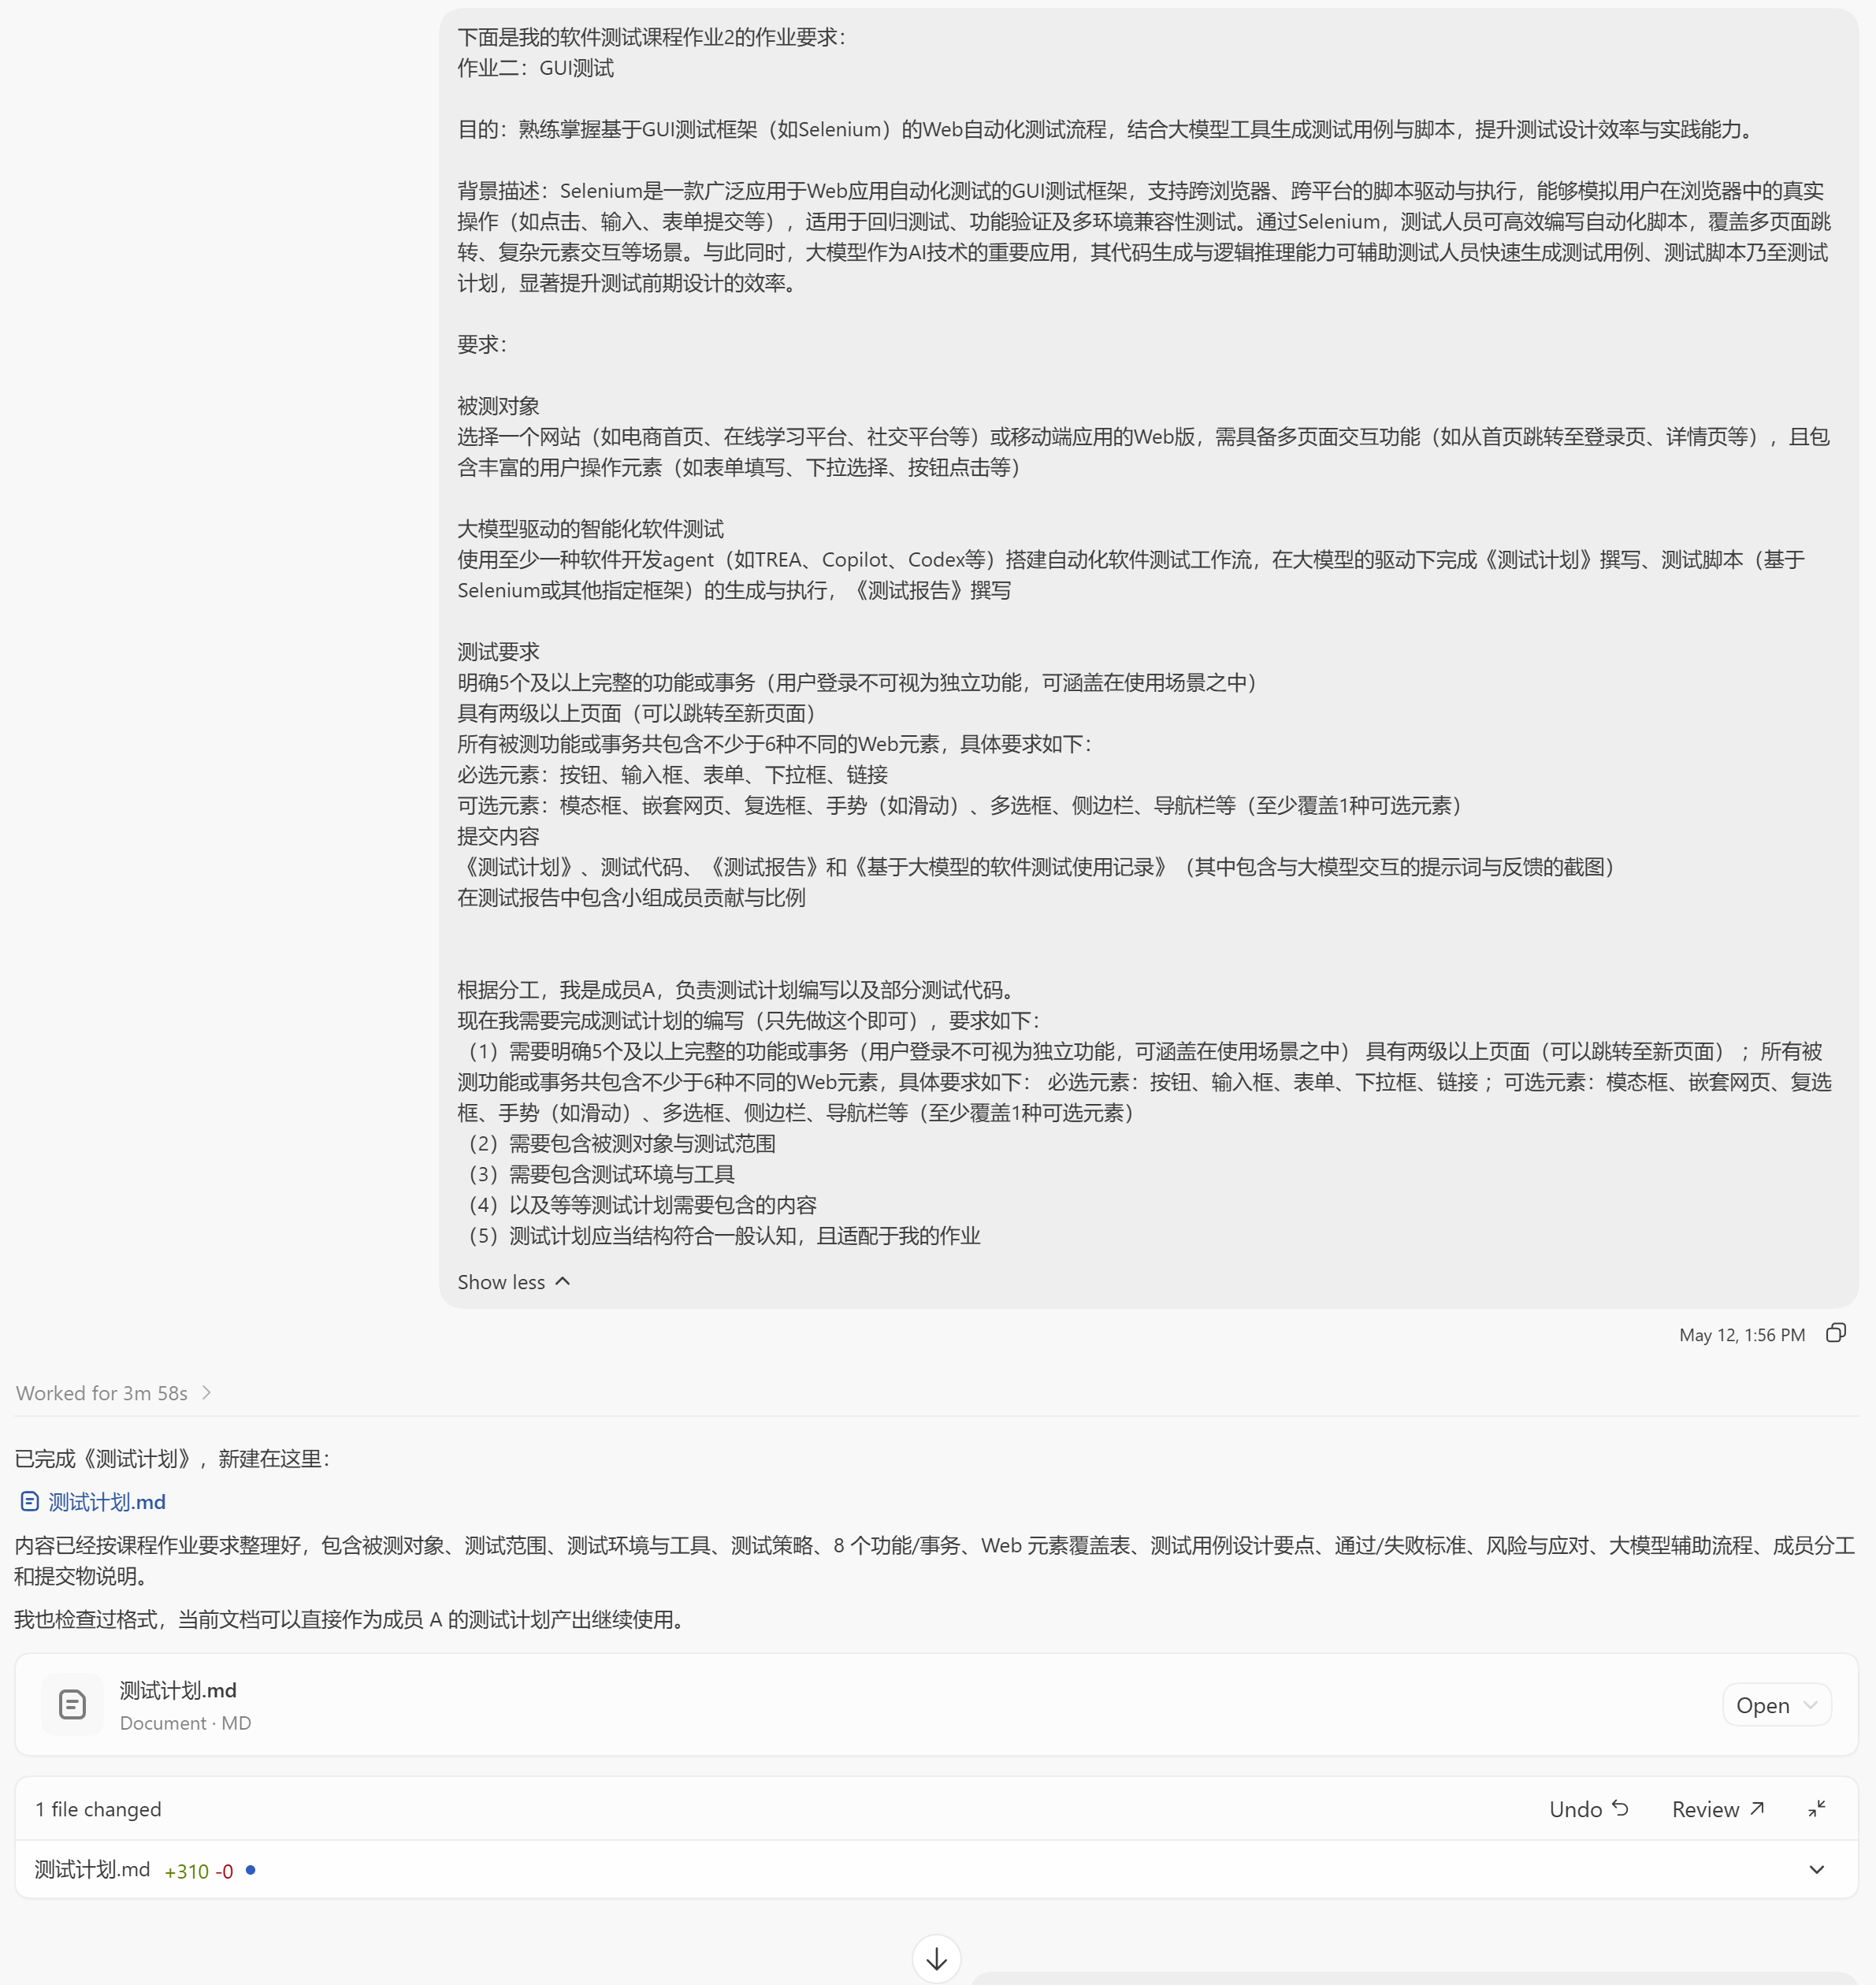
\includegraphics[width=0.92\textwidth]{member_a/测试计划启动.png}
\caption{向大模型说明作业要求和个人分工，启动测试计划编写。}
\end{figure}

\begin{figure}[H]
\centering
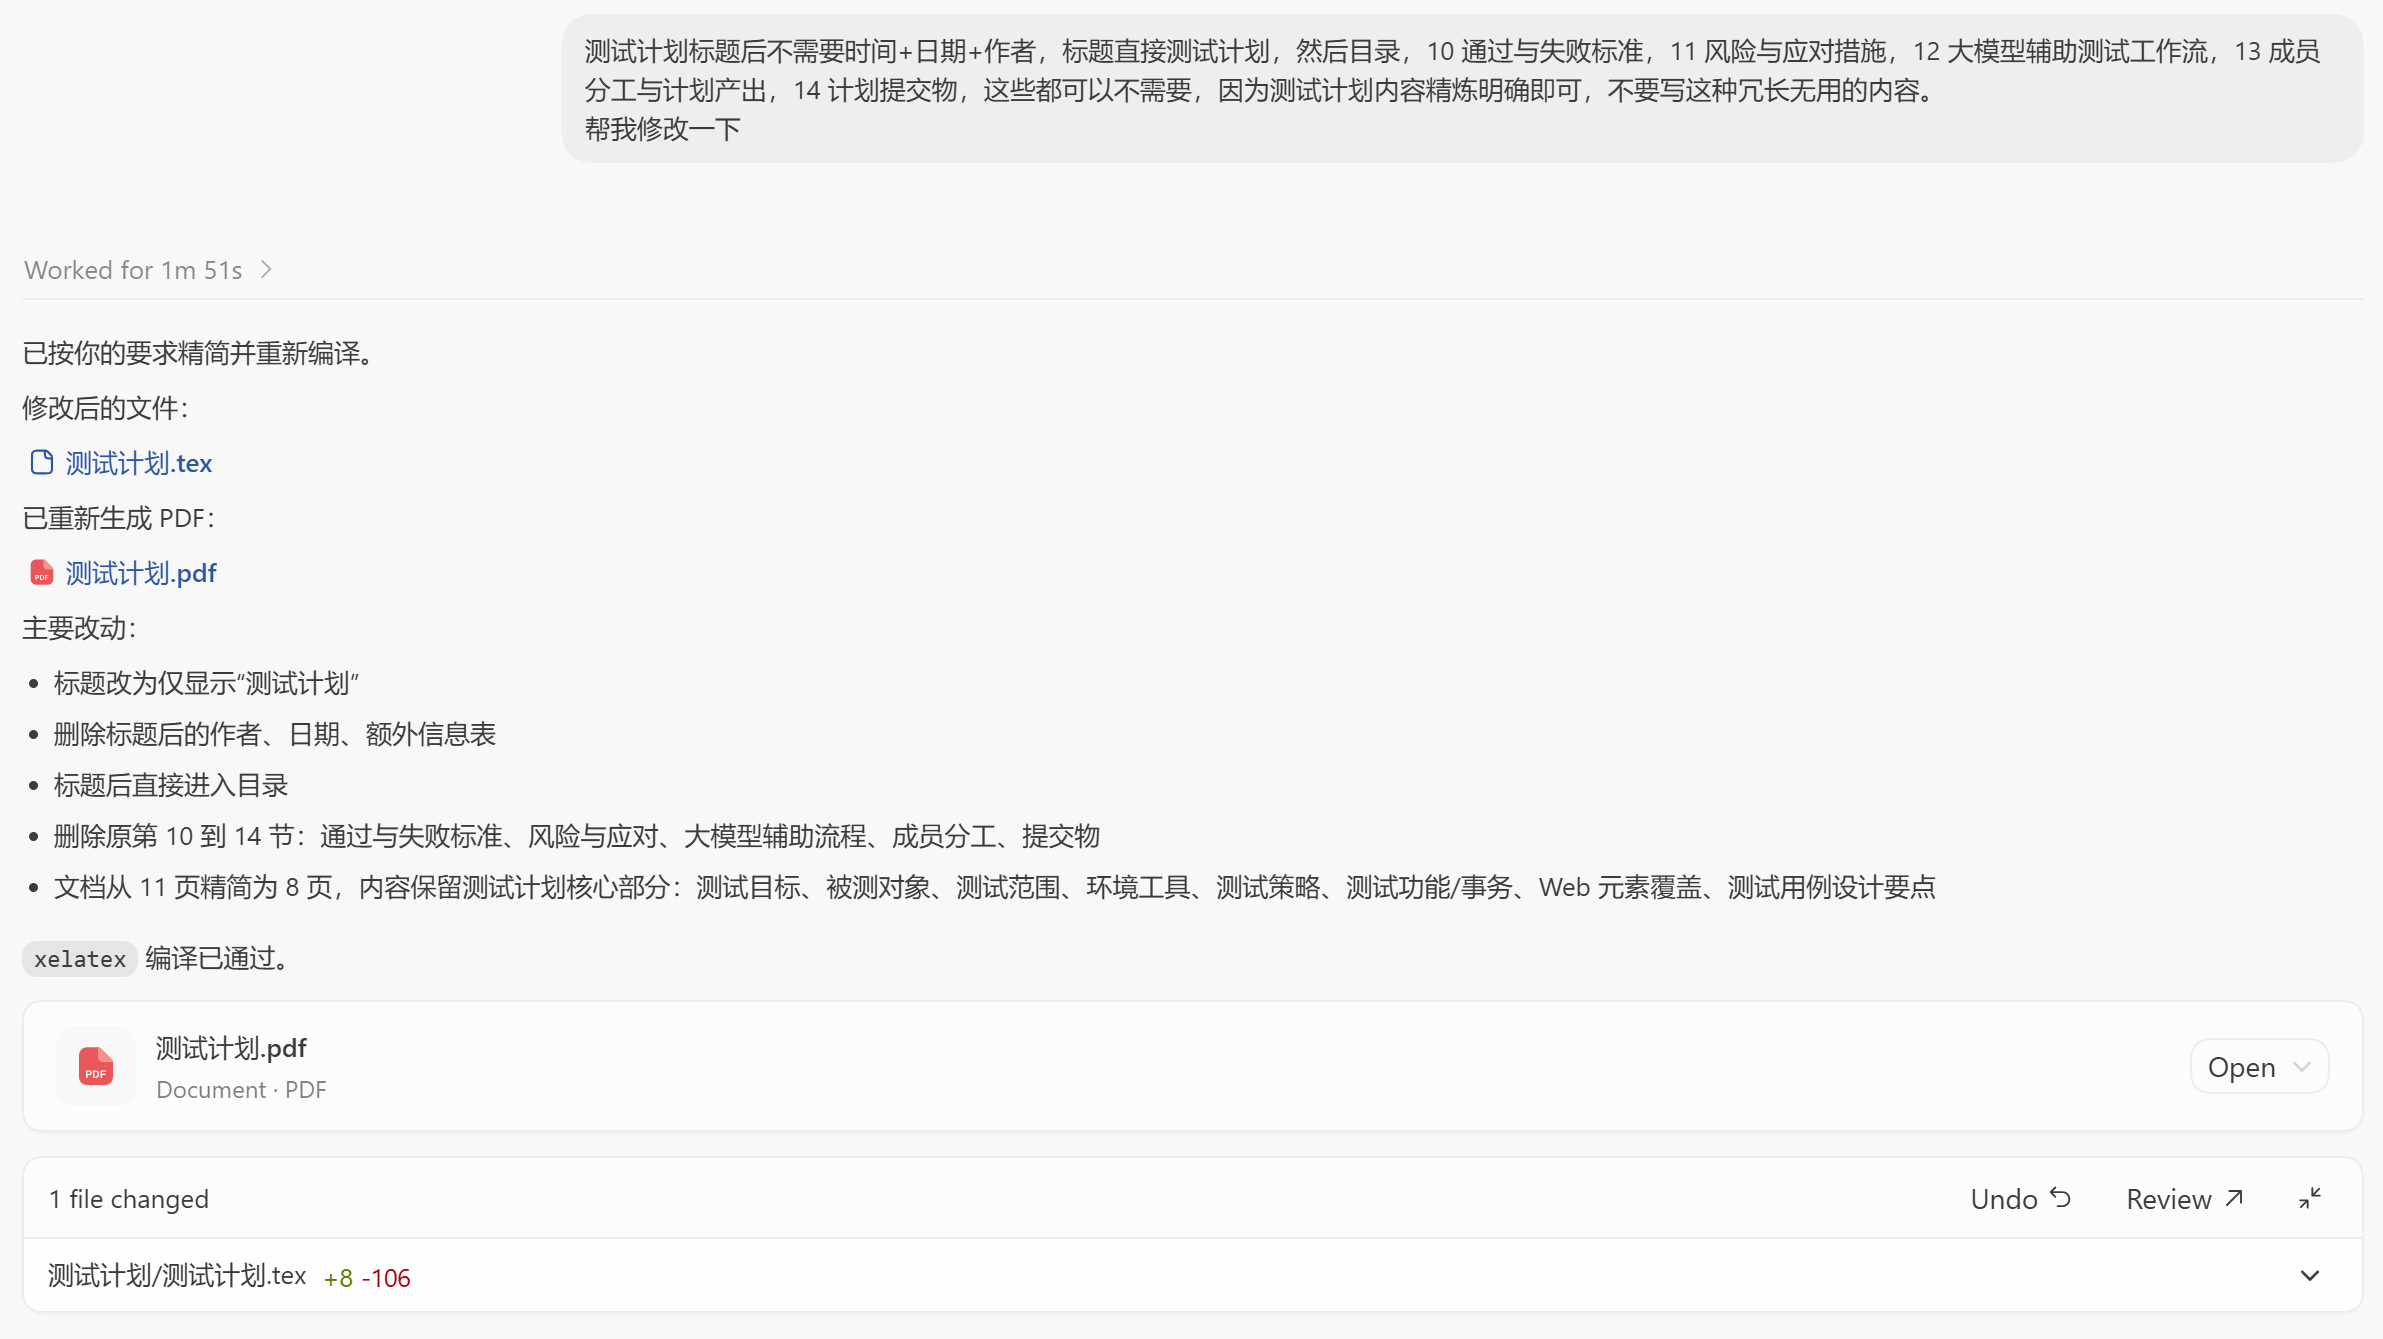
\includegraphics[width=0.92\textwidth]{member_a/测试计划修改.png}
\caption{根据课程要求和报告结构，对测试计划内容进行精简和调整。}
\end{figure}

\begin{figure}[H]
\centering
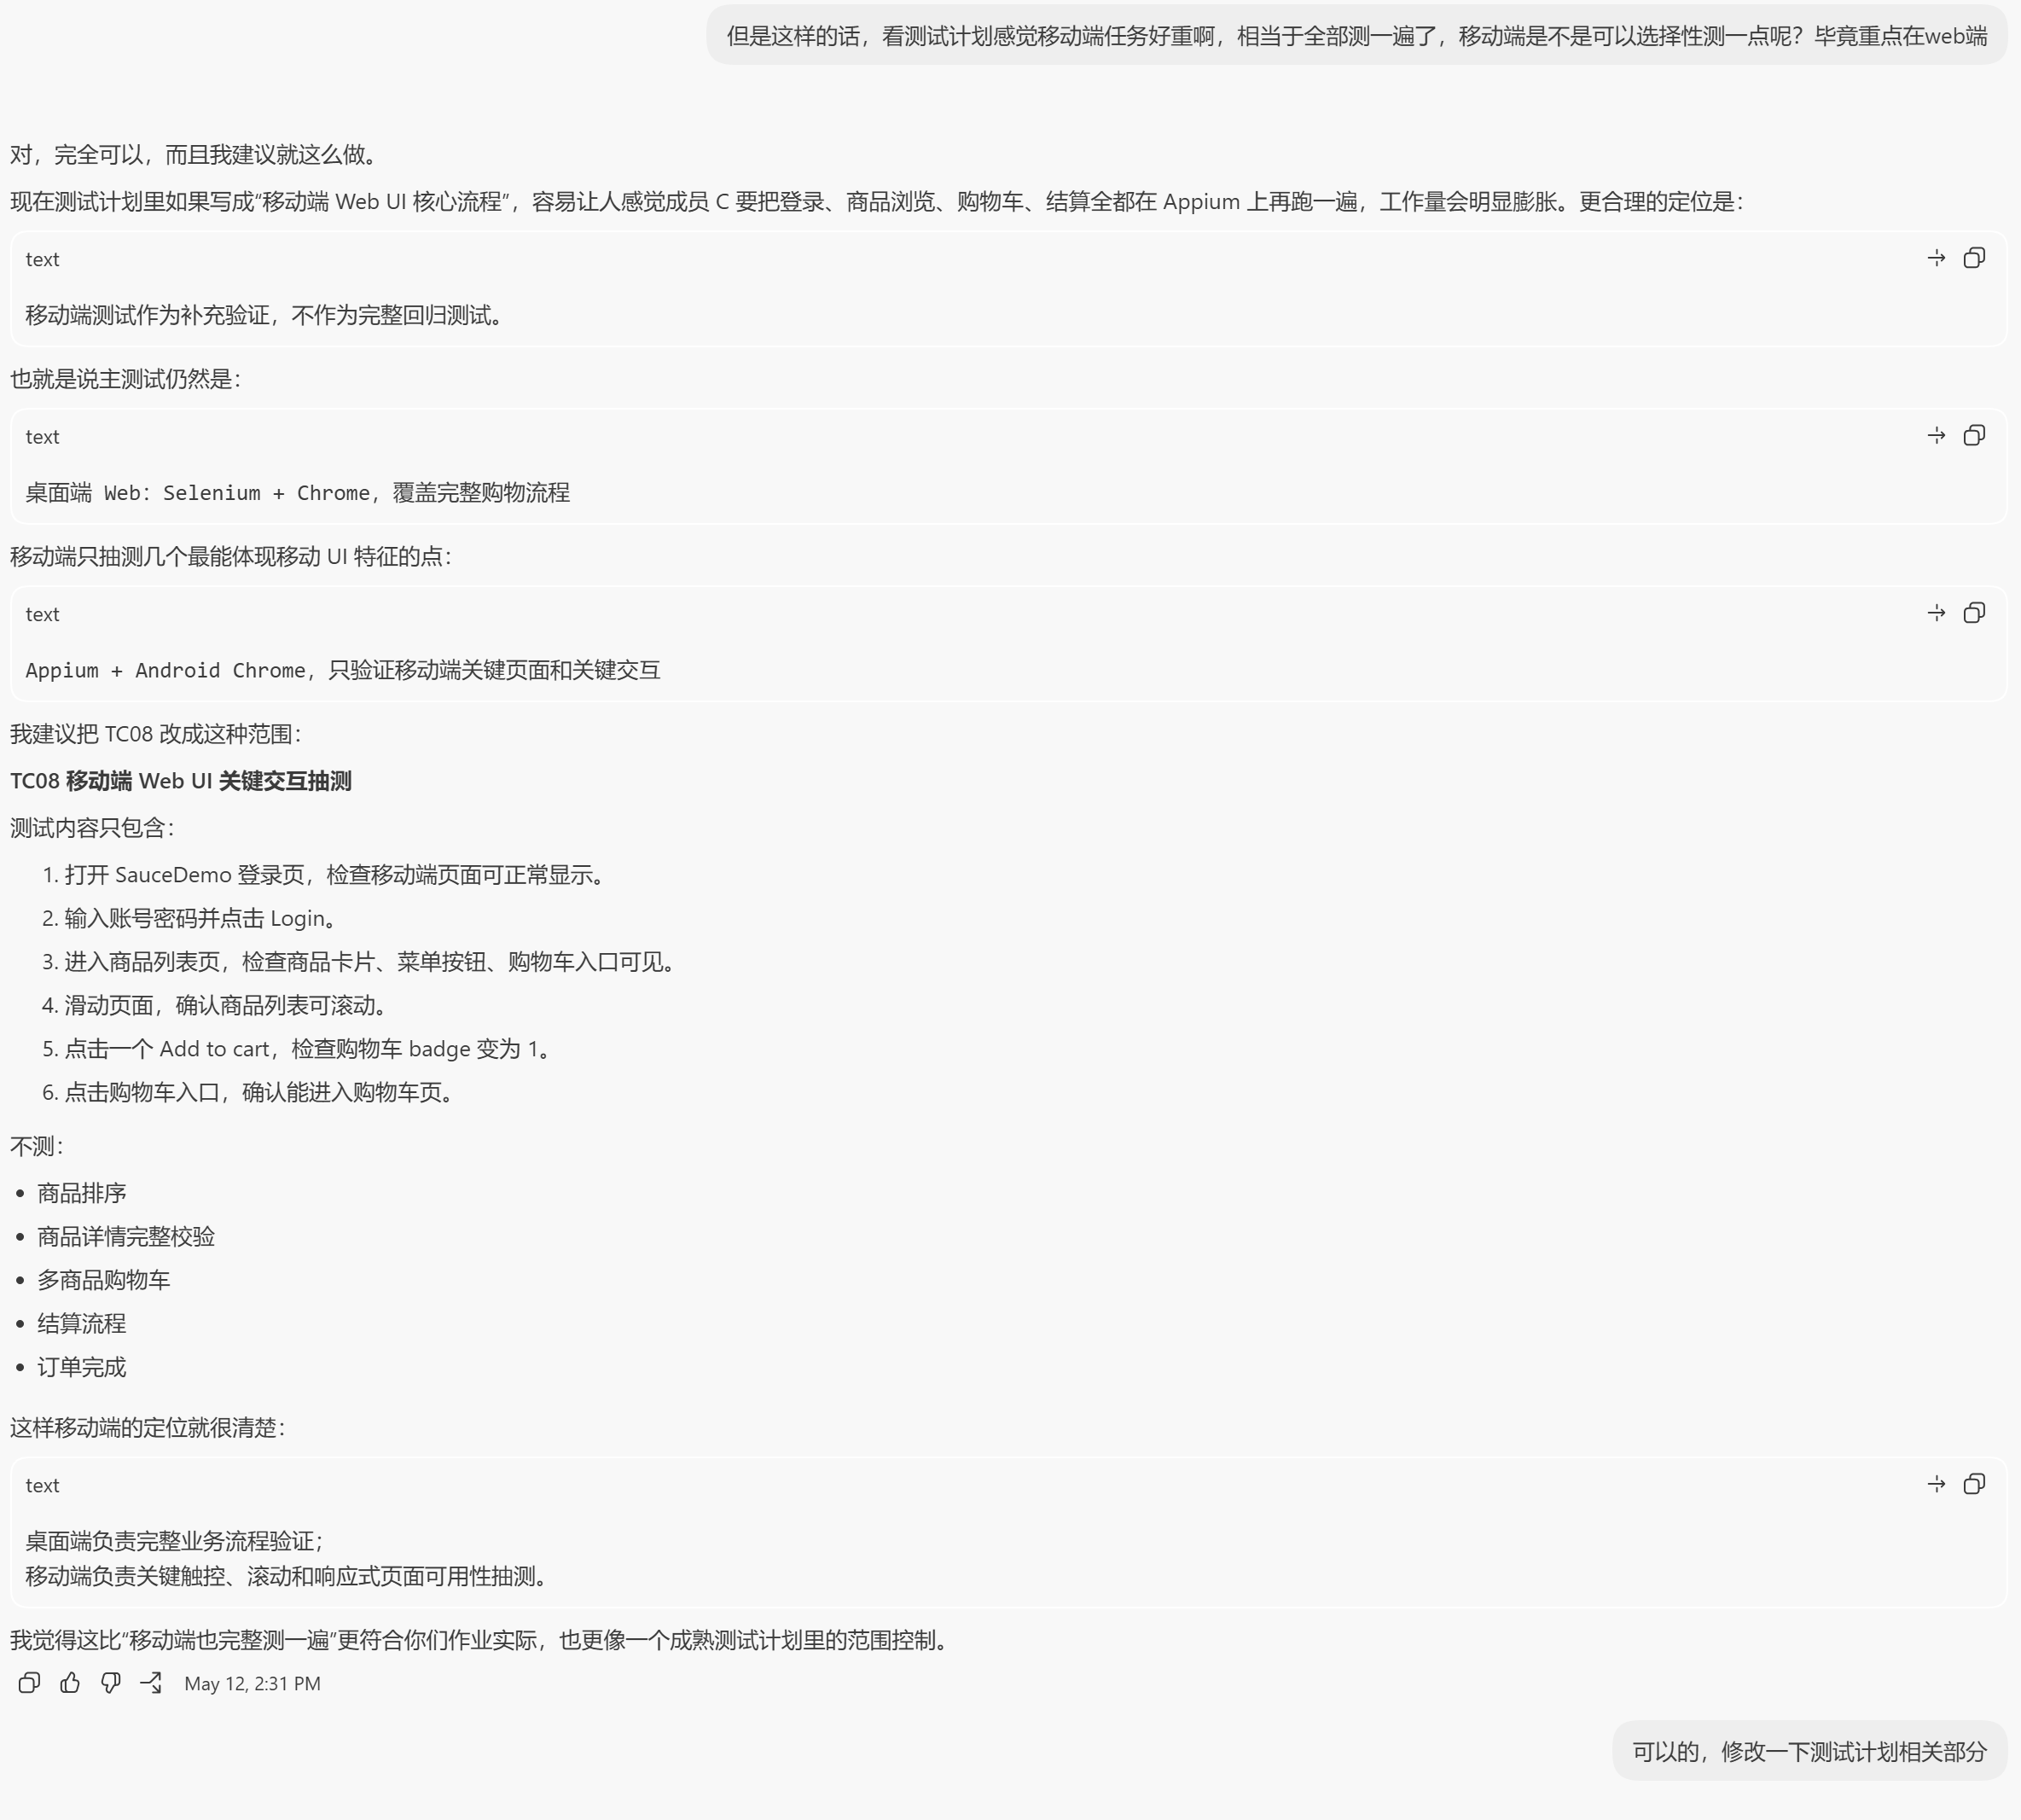
\includegraphics[width=0.92\textwidth]{member_a/测试计划进一步调整.png}
\caption{进一步讨论移动端 Web UI 测试范围、环境搭建方式和回退方案。}
\end{figure}

\subsection{测试代码生成与执行}

\begin{figure}[H]
\centering
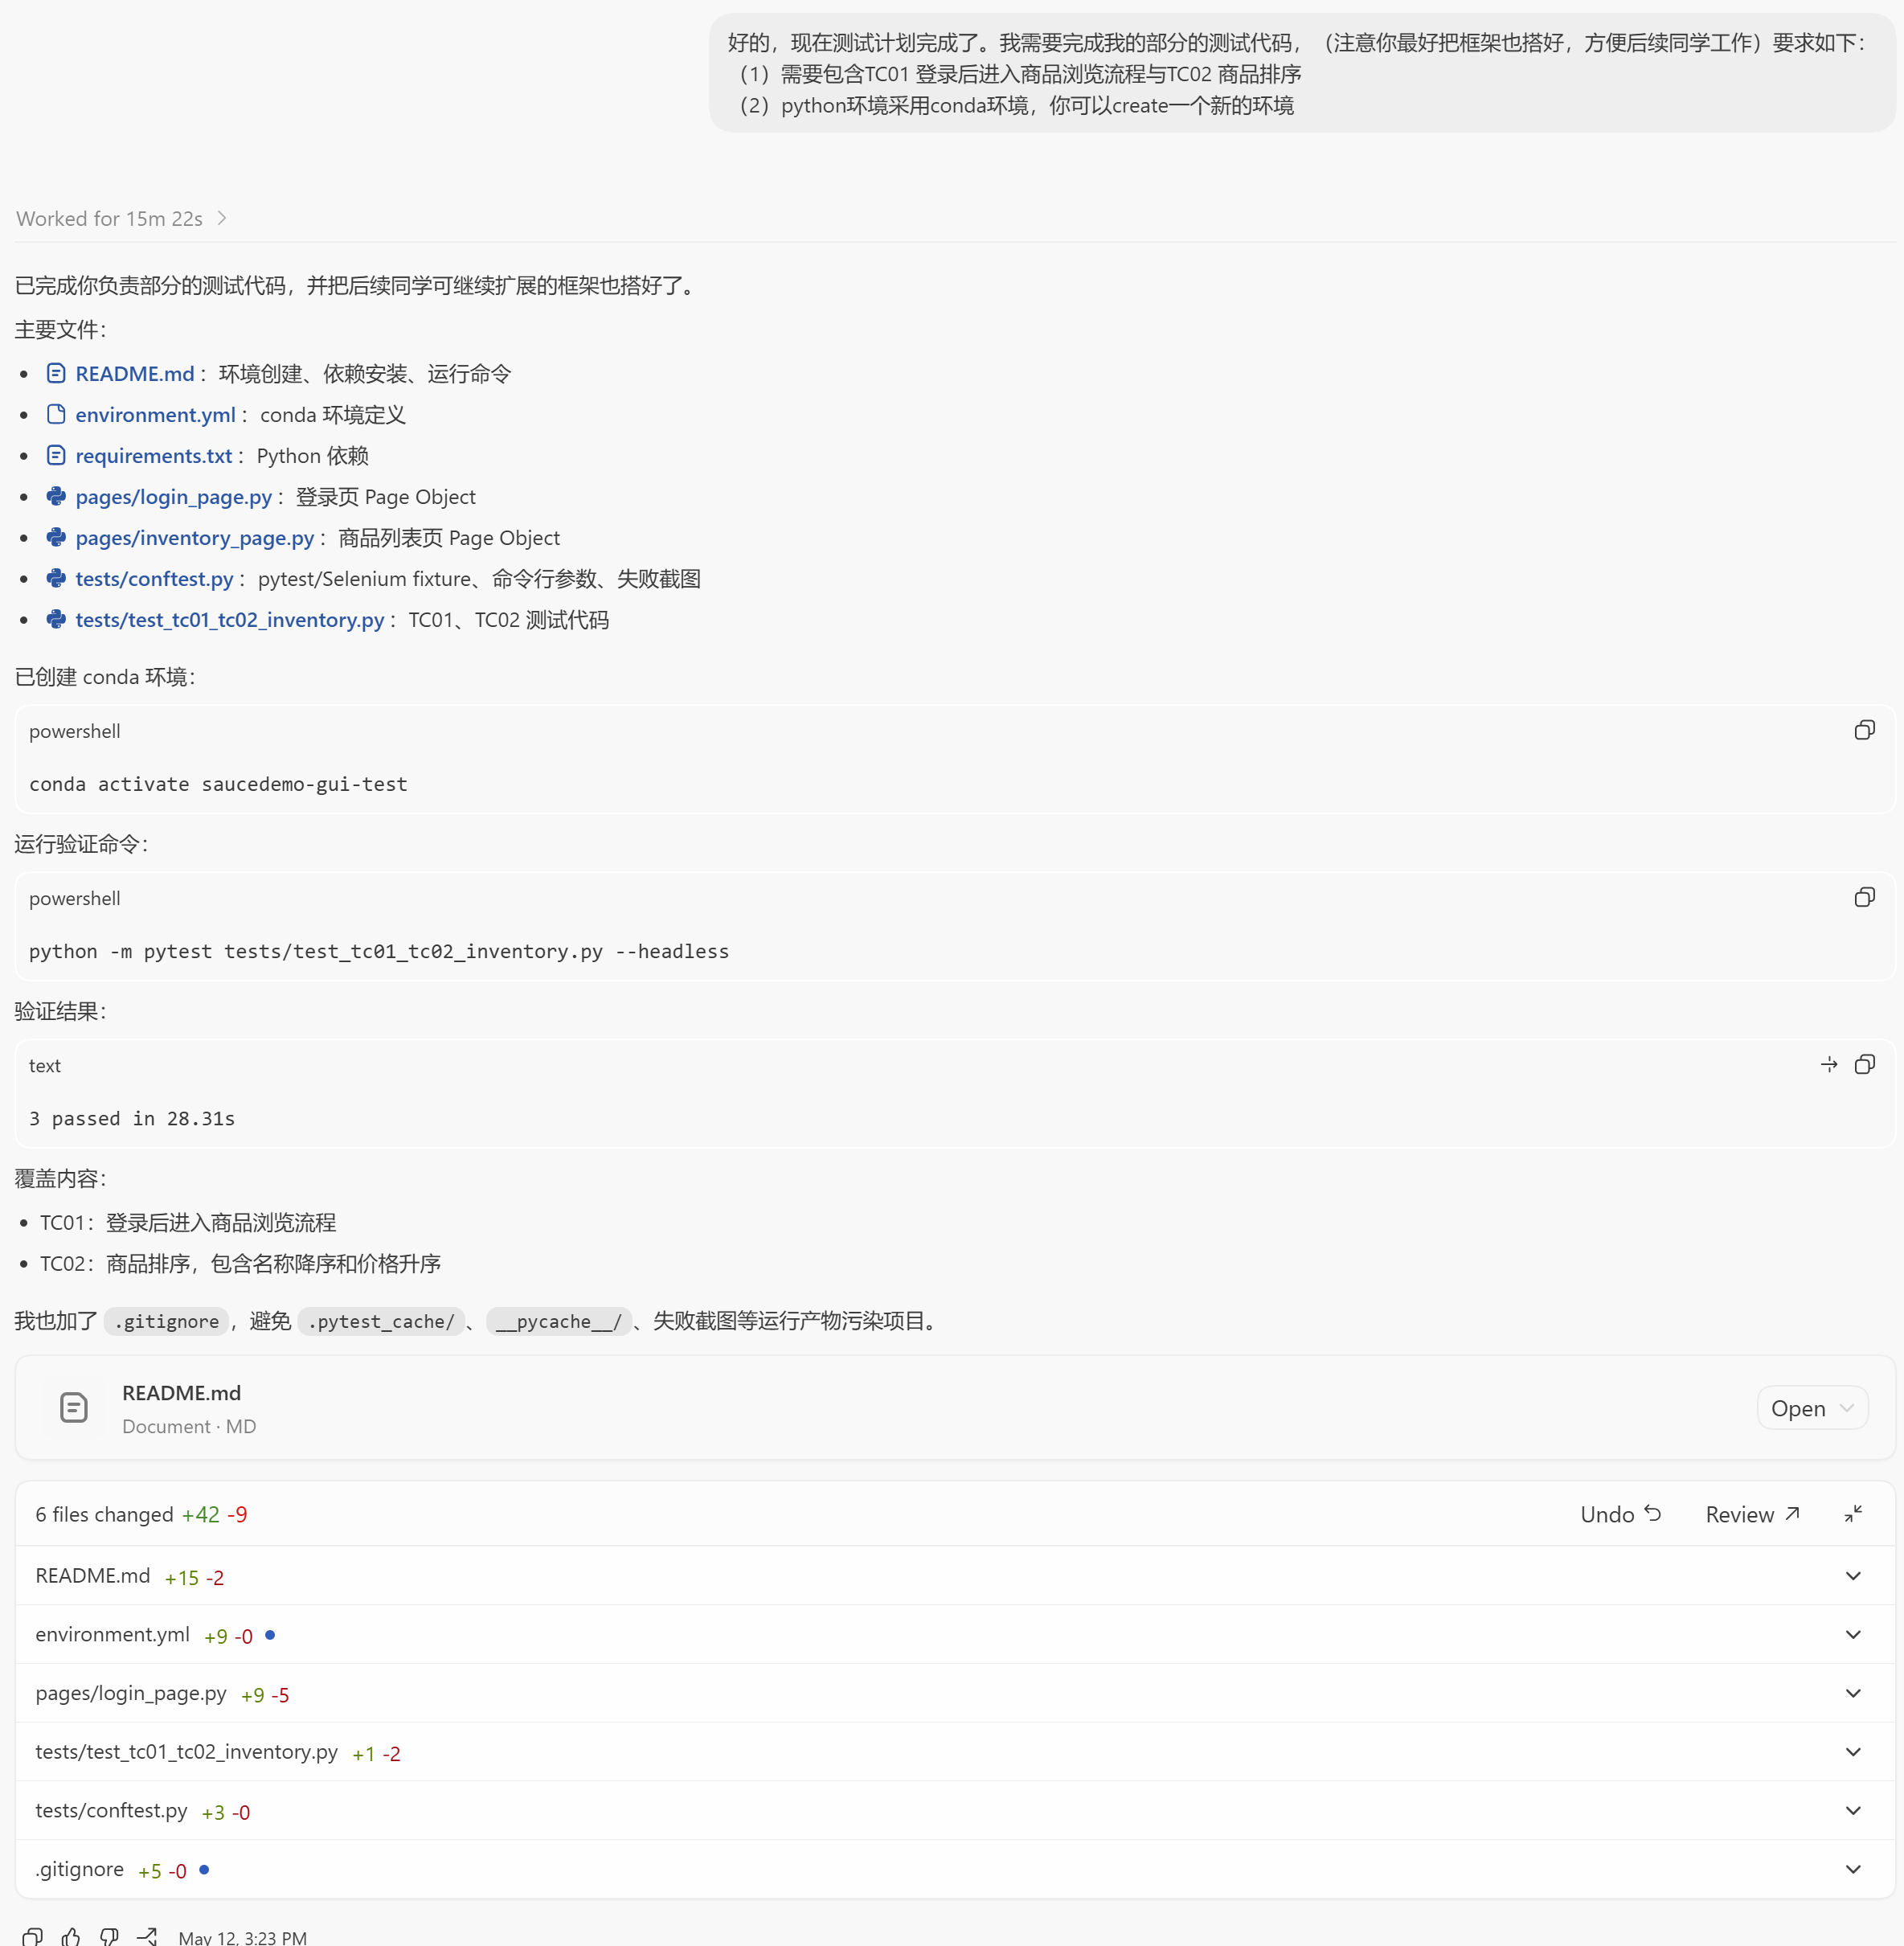
\includegraphics[width=0.92\textwidth]{member_a/测试代码启动.png}
\caption{要求大模型搭建 Selenium 自动化测试框架并实现 TC01、TC02 测试脚本。}
\end{figure}

\subsection{测试报告编写与修改}

\begin{figure}[H]
\centering
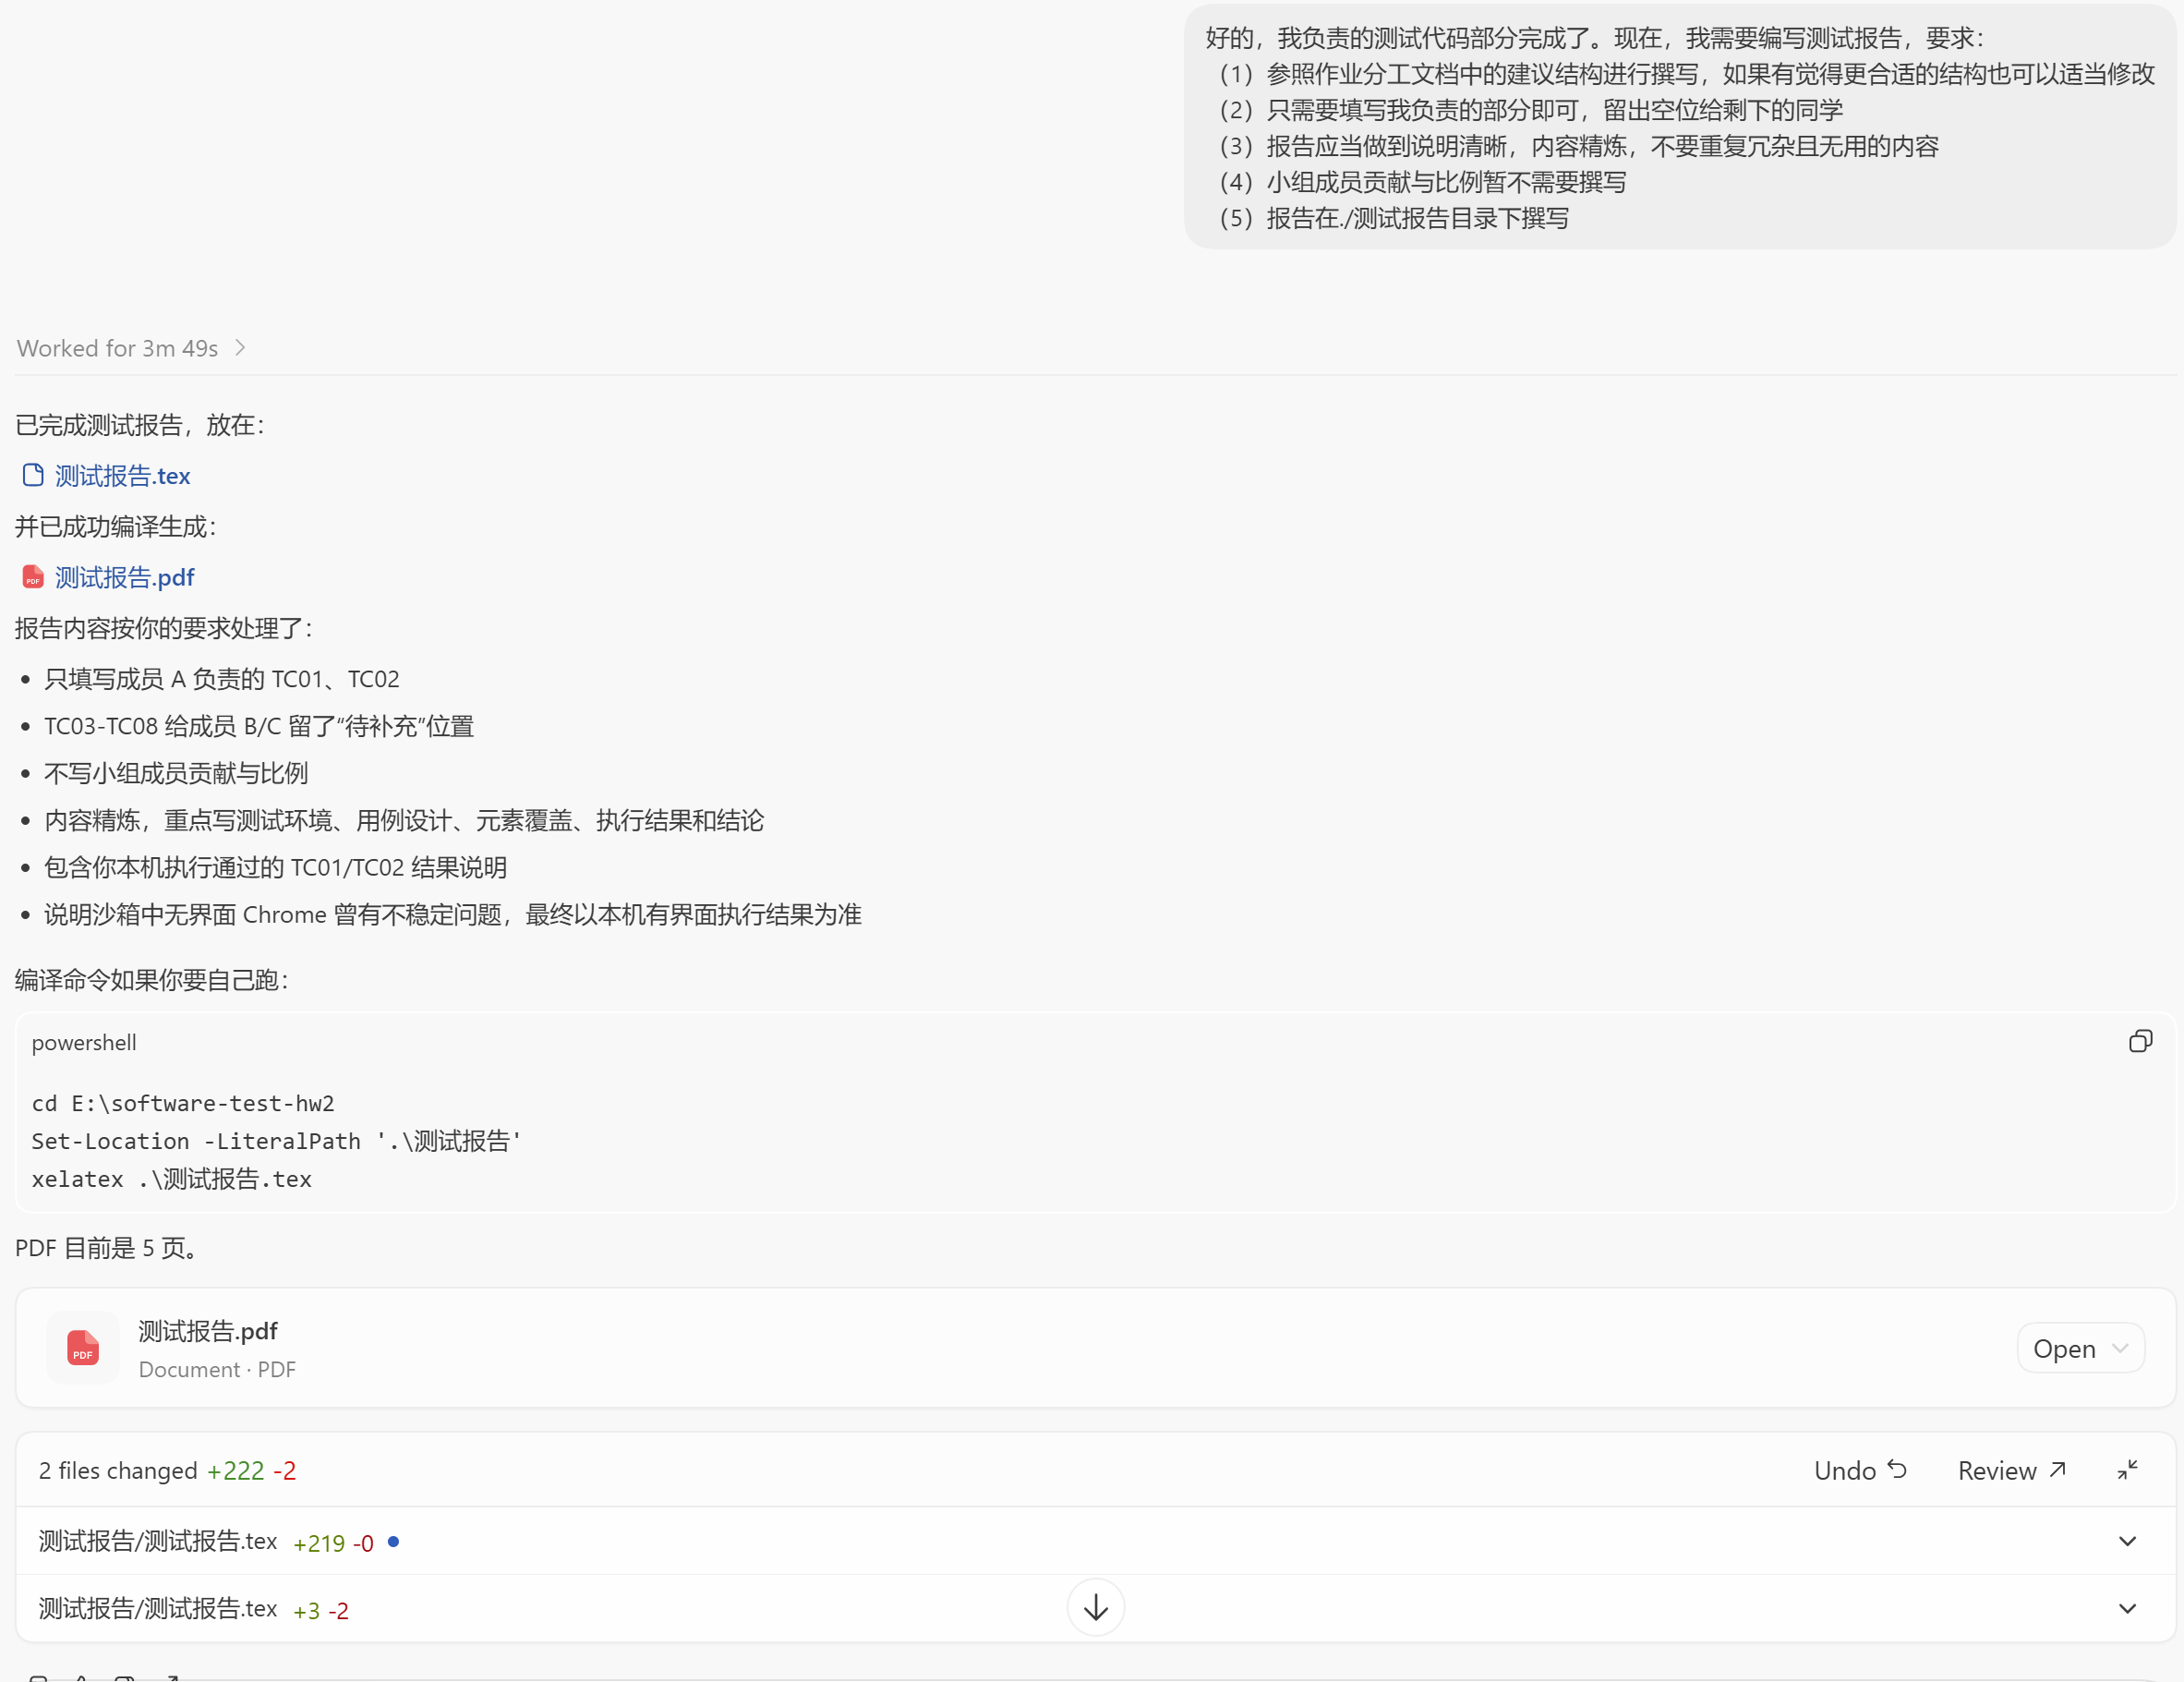
\includegraphics[width=0.92\textwidth]{member_a/测试报告启动.png}
\caption{向大模型说明测试报告撰写要求，并生成报告初稿。}
\end{figure}

\begin{figure}[H]
\centering
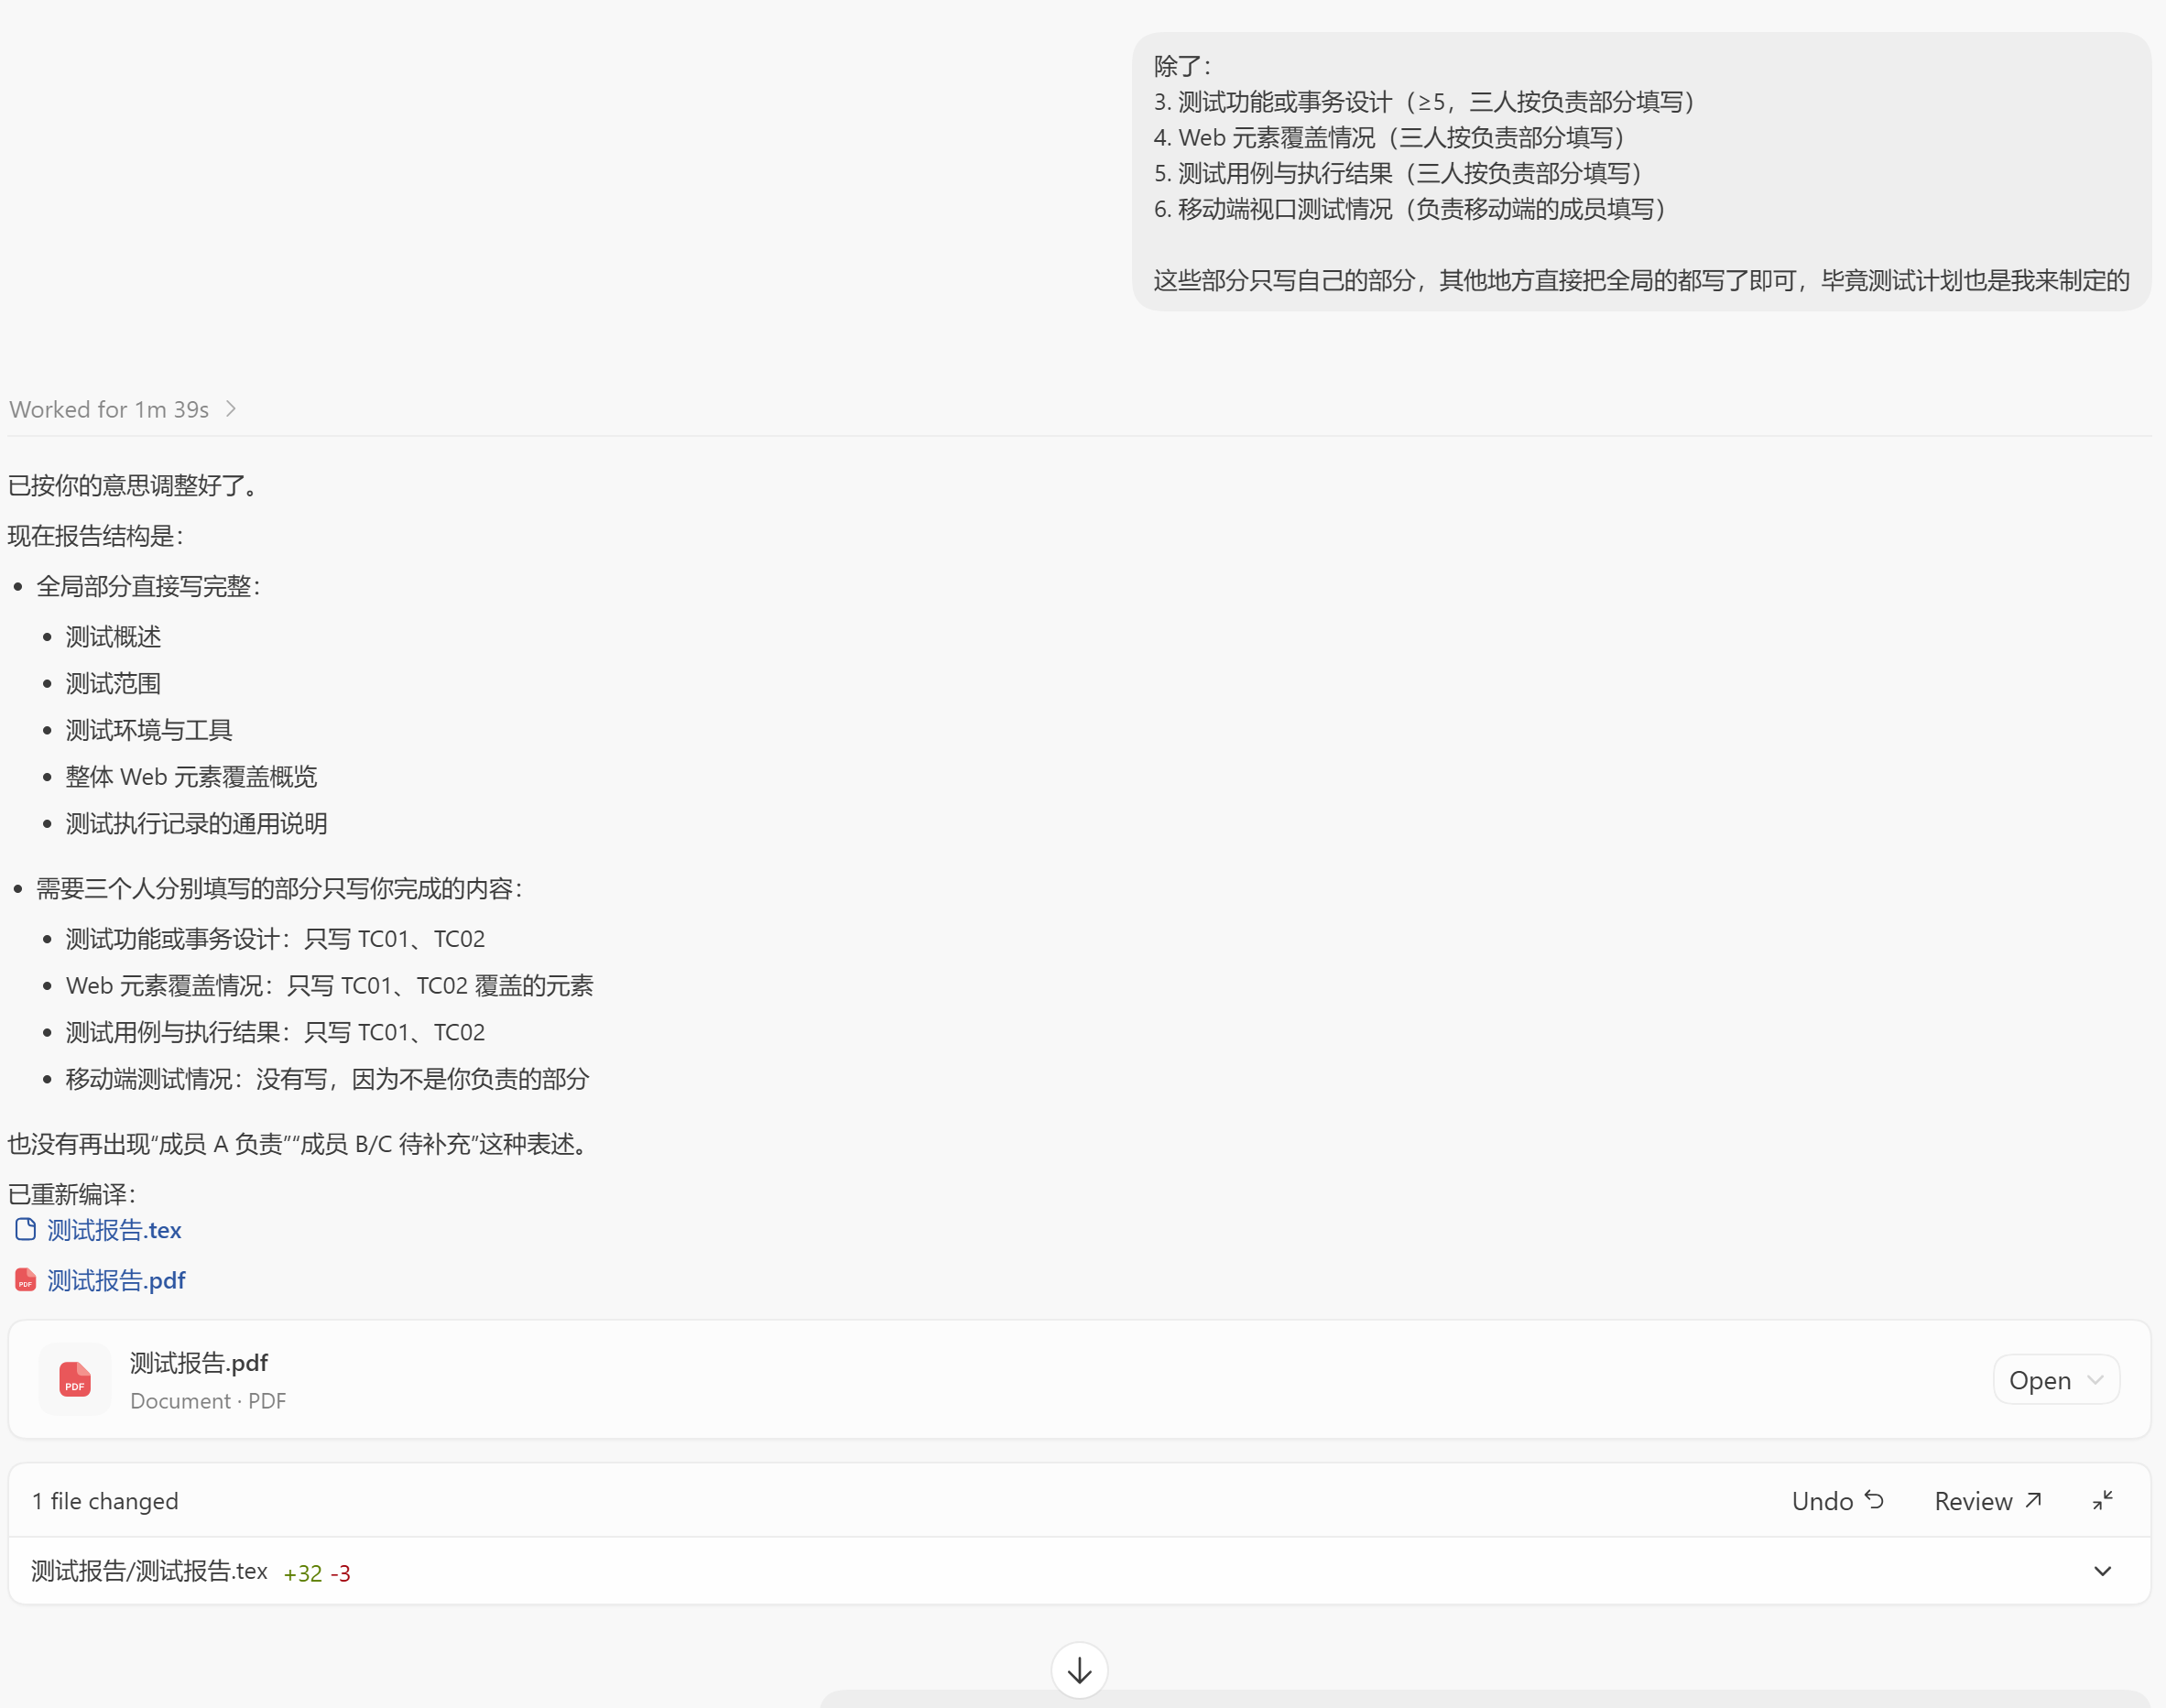
\includegraphics[width=0.92\textwidth]{member_a/测试报告修改.png}
\caption{围绕报告表述方式、章节划分和成员内容边界进行修改。}
\end{figure}

\begin{figure}[H]
\centering
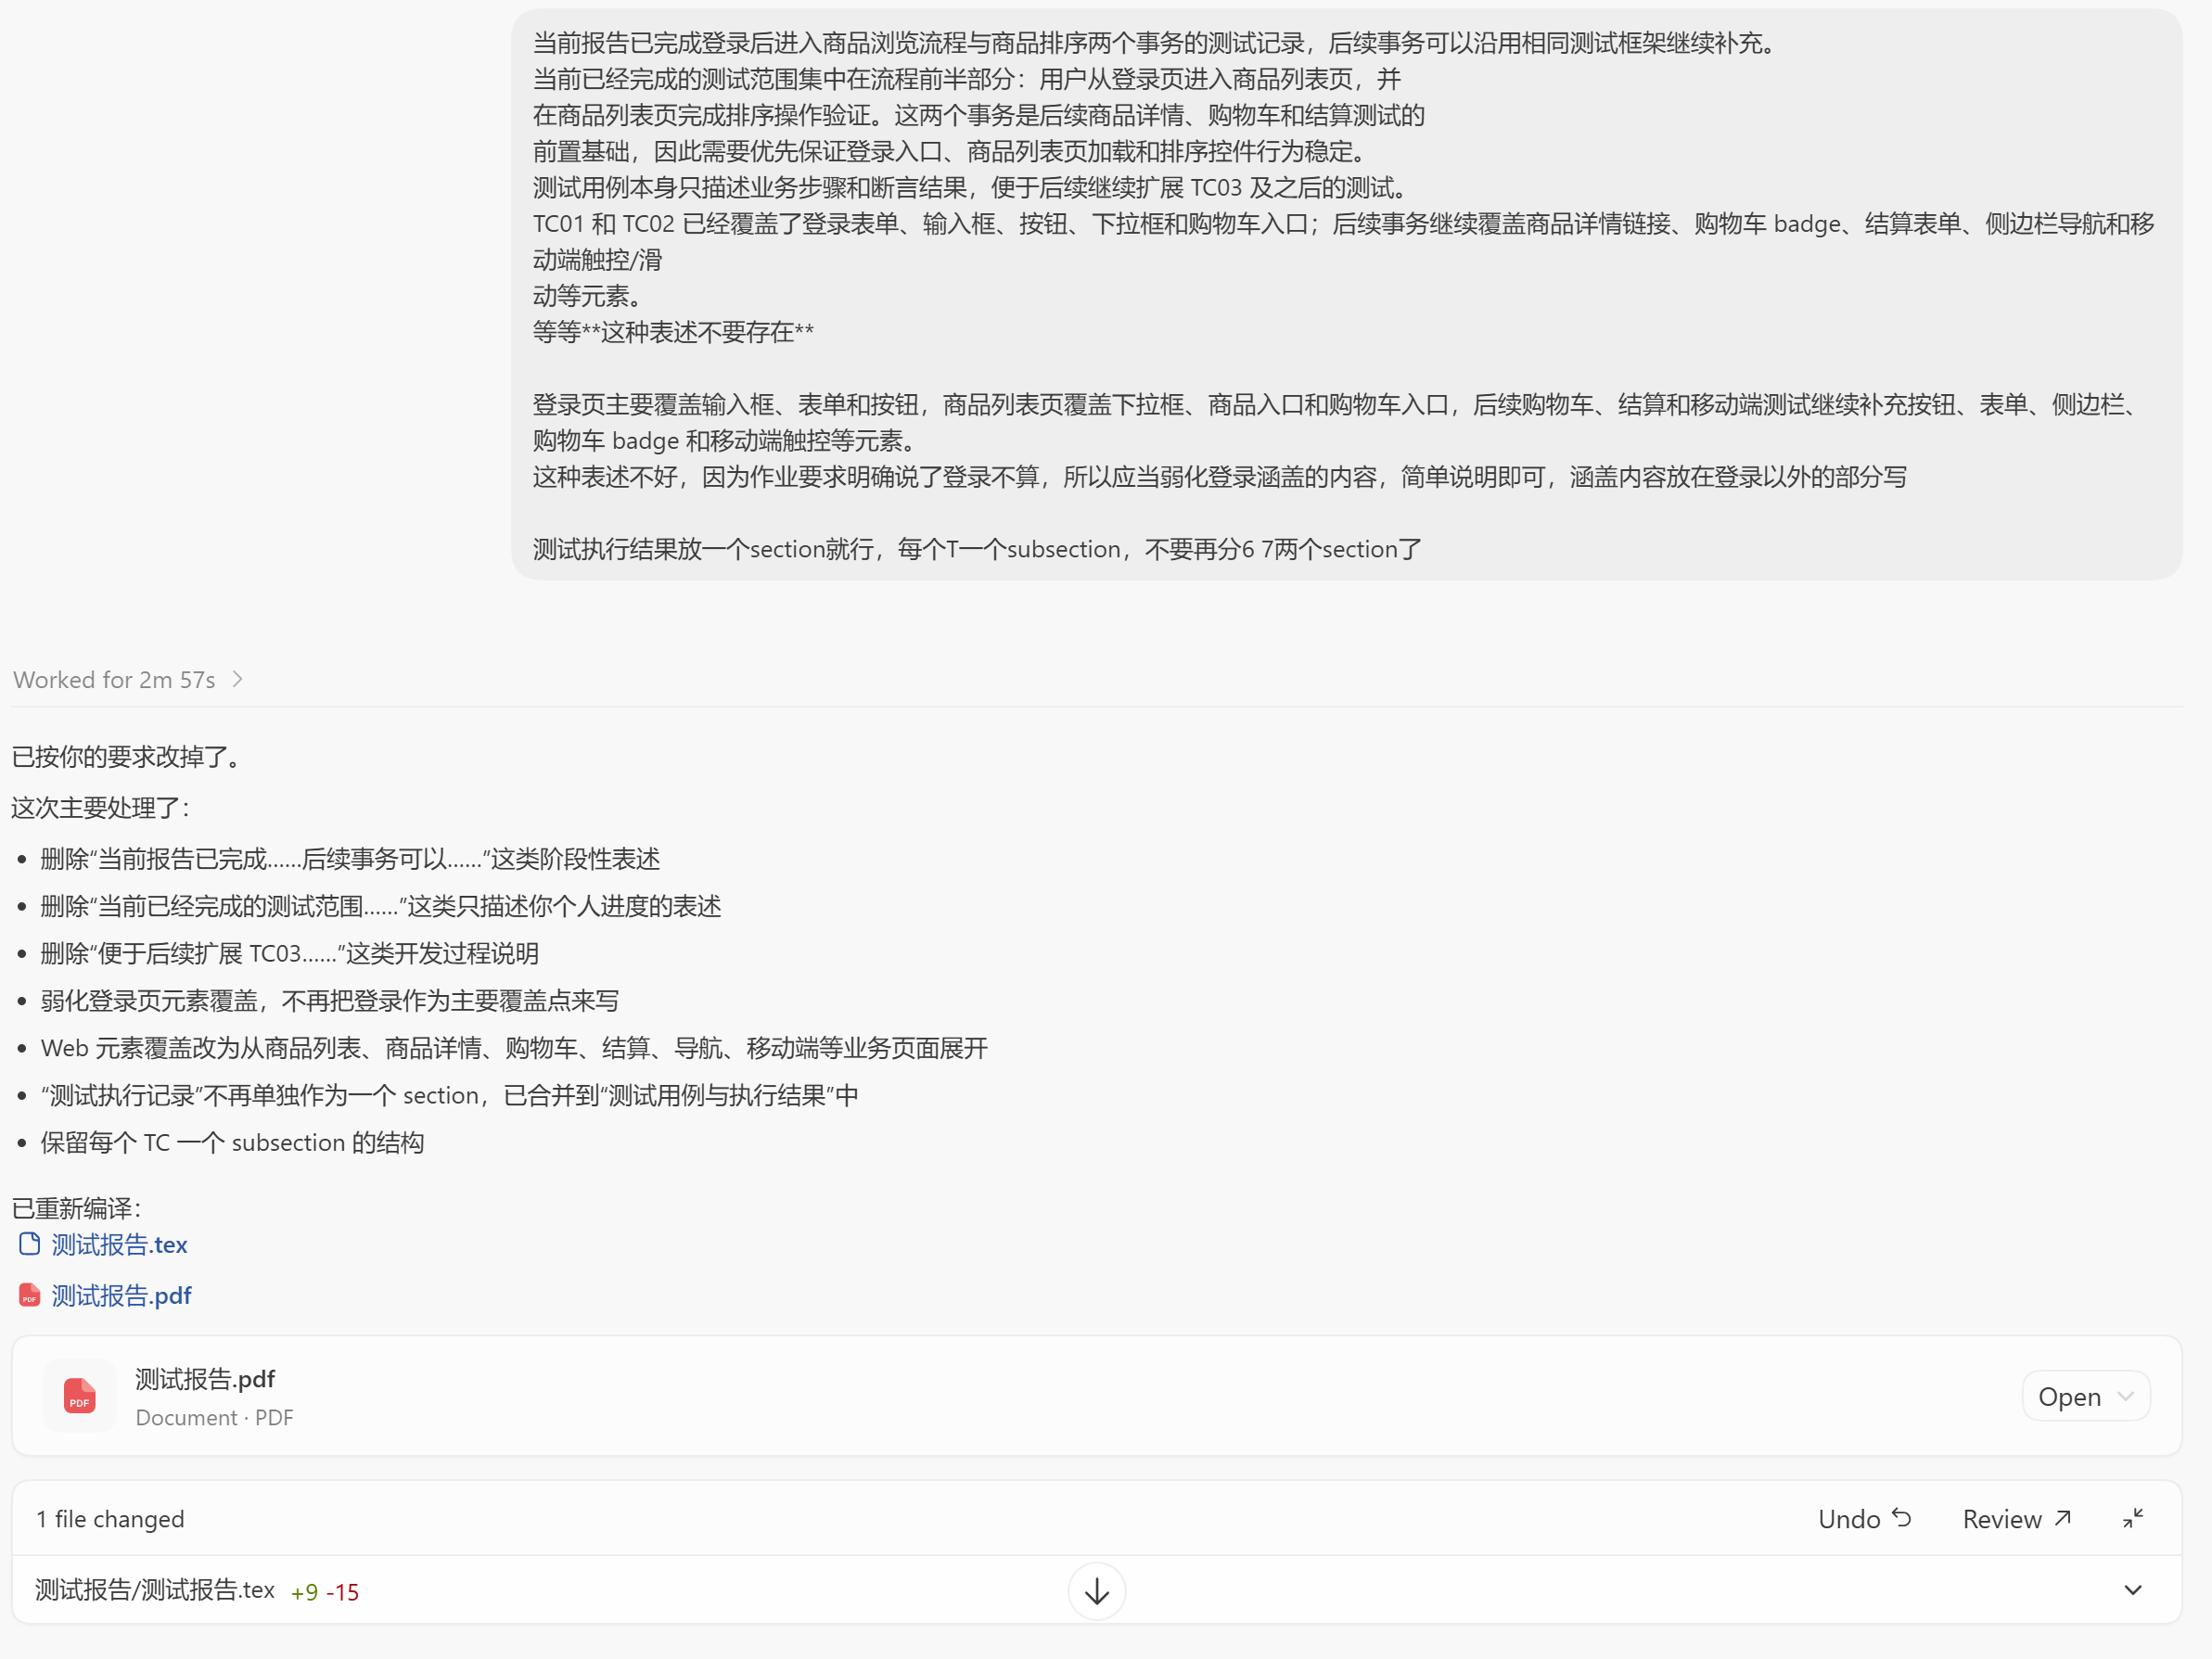
\includegraphics[width=0.92\textwidth]{member_a/测试报告修改2.png}
\caption{继续优化测试报告中的元素覆盖表、执行结果截图和成员贡献部分。}
\end{figure}

\section{成员B使用记录}

\subsection{测试代码生成与执行}

\begin{figure}[H]
\centering
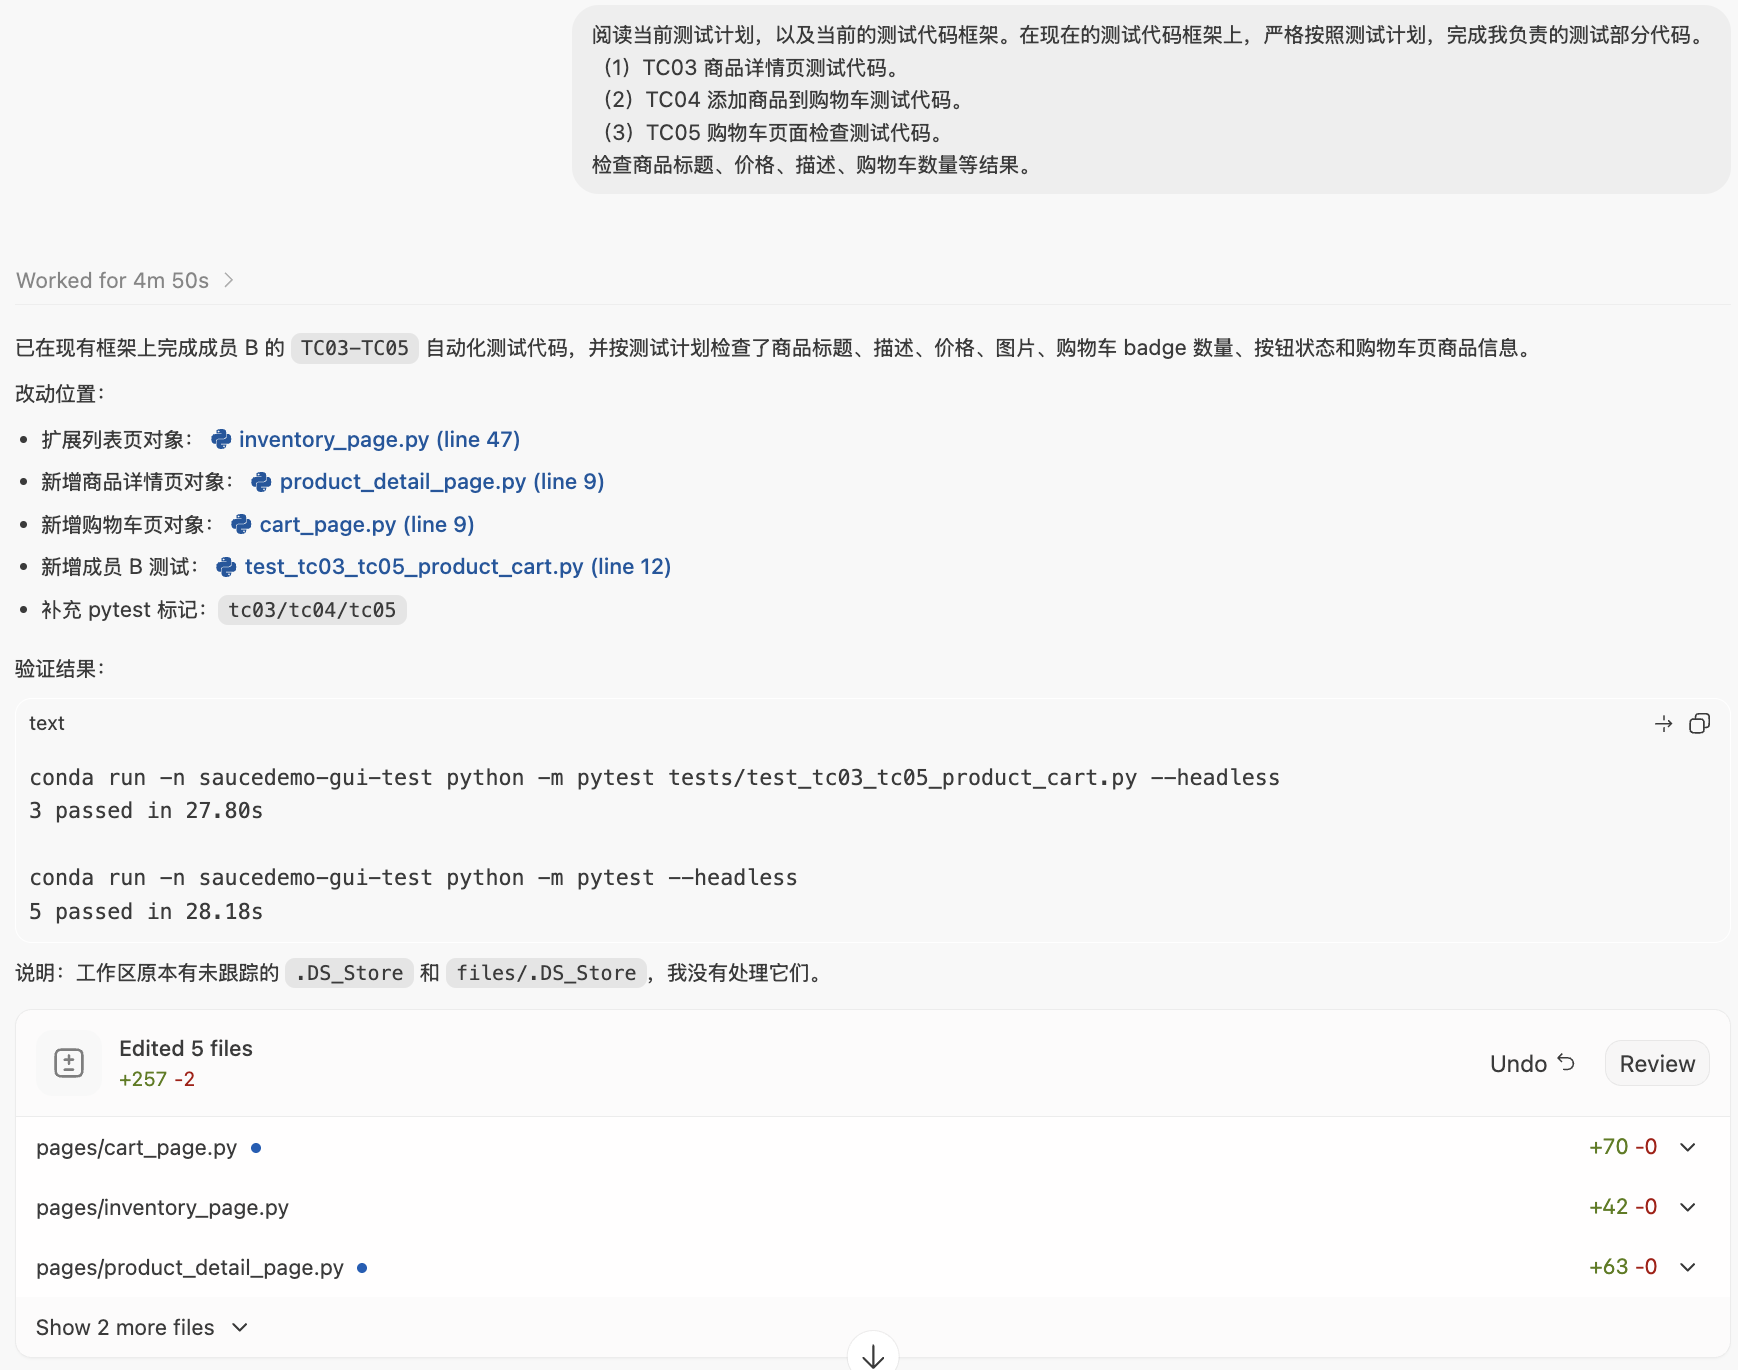
\includegraphics[width=0.92\textwidth]{member_b/测试代码生成.png}
\caption{向大模型说明成员 B 分工和测试计划要求，生成 TC03、TC04、TC05 商品详情与购物车测试代码。}
\end{figure}

\begin{figure}[H]
\centering
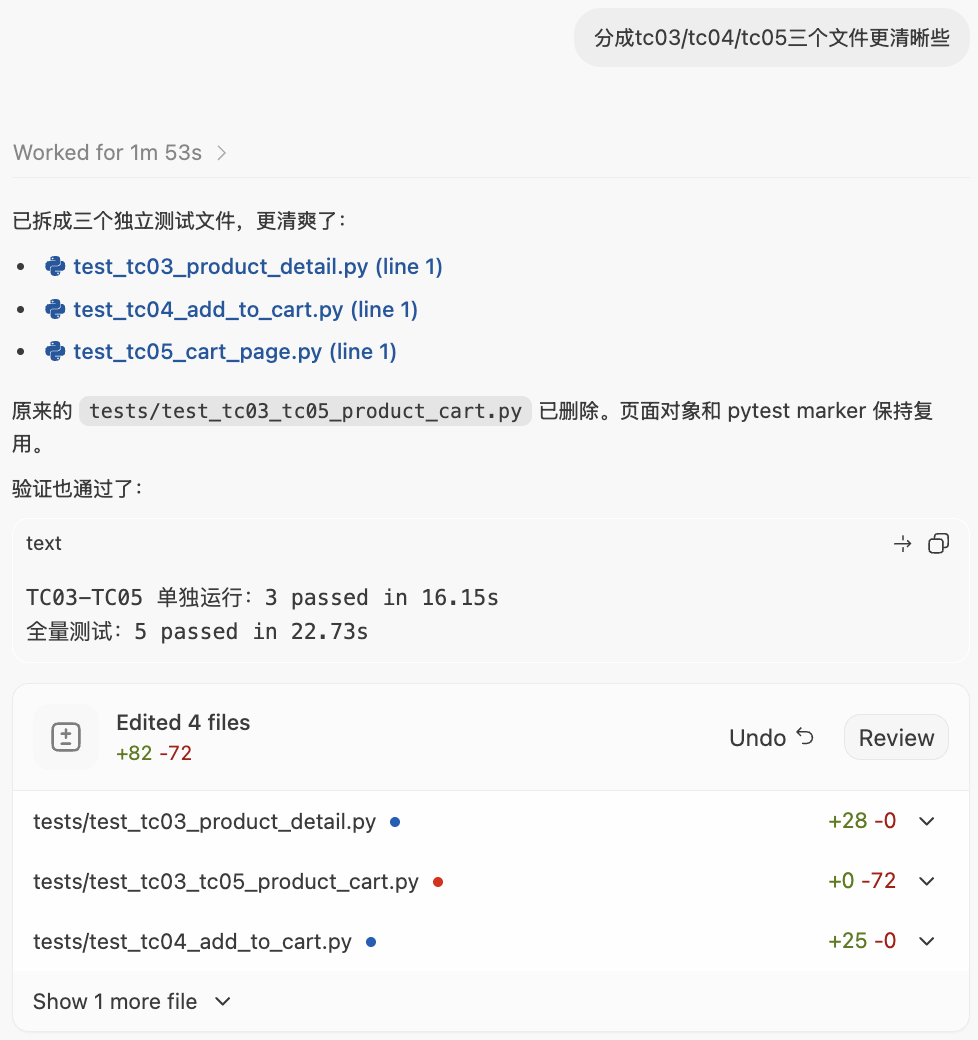
\includegraphics[width=0.92\textwidth]{member_b/测试代码调整.png}
\caption{根据代码组织清晰度要求，将成员 B 测试拆分为 TC03、TC04、TC05 三个独立测试文件，并重新运行验证。}
\end{figure}

\subsection{测试报告编写与修改}

\begin{figure}[H]
\centering
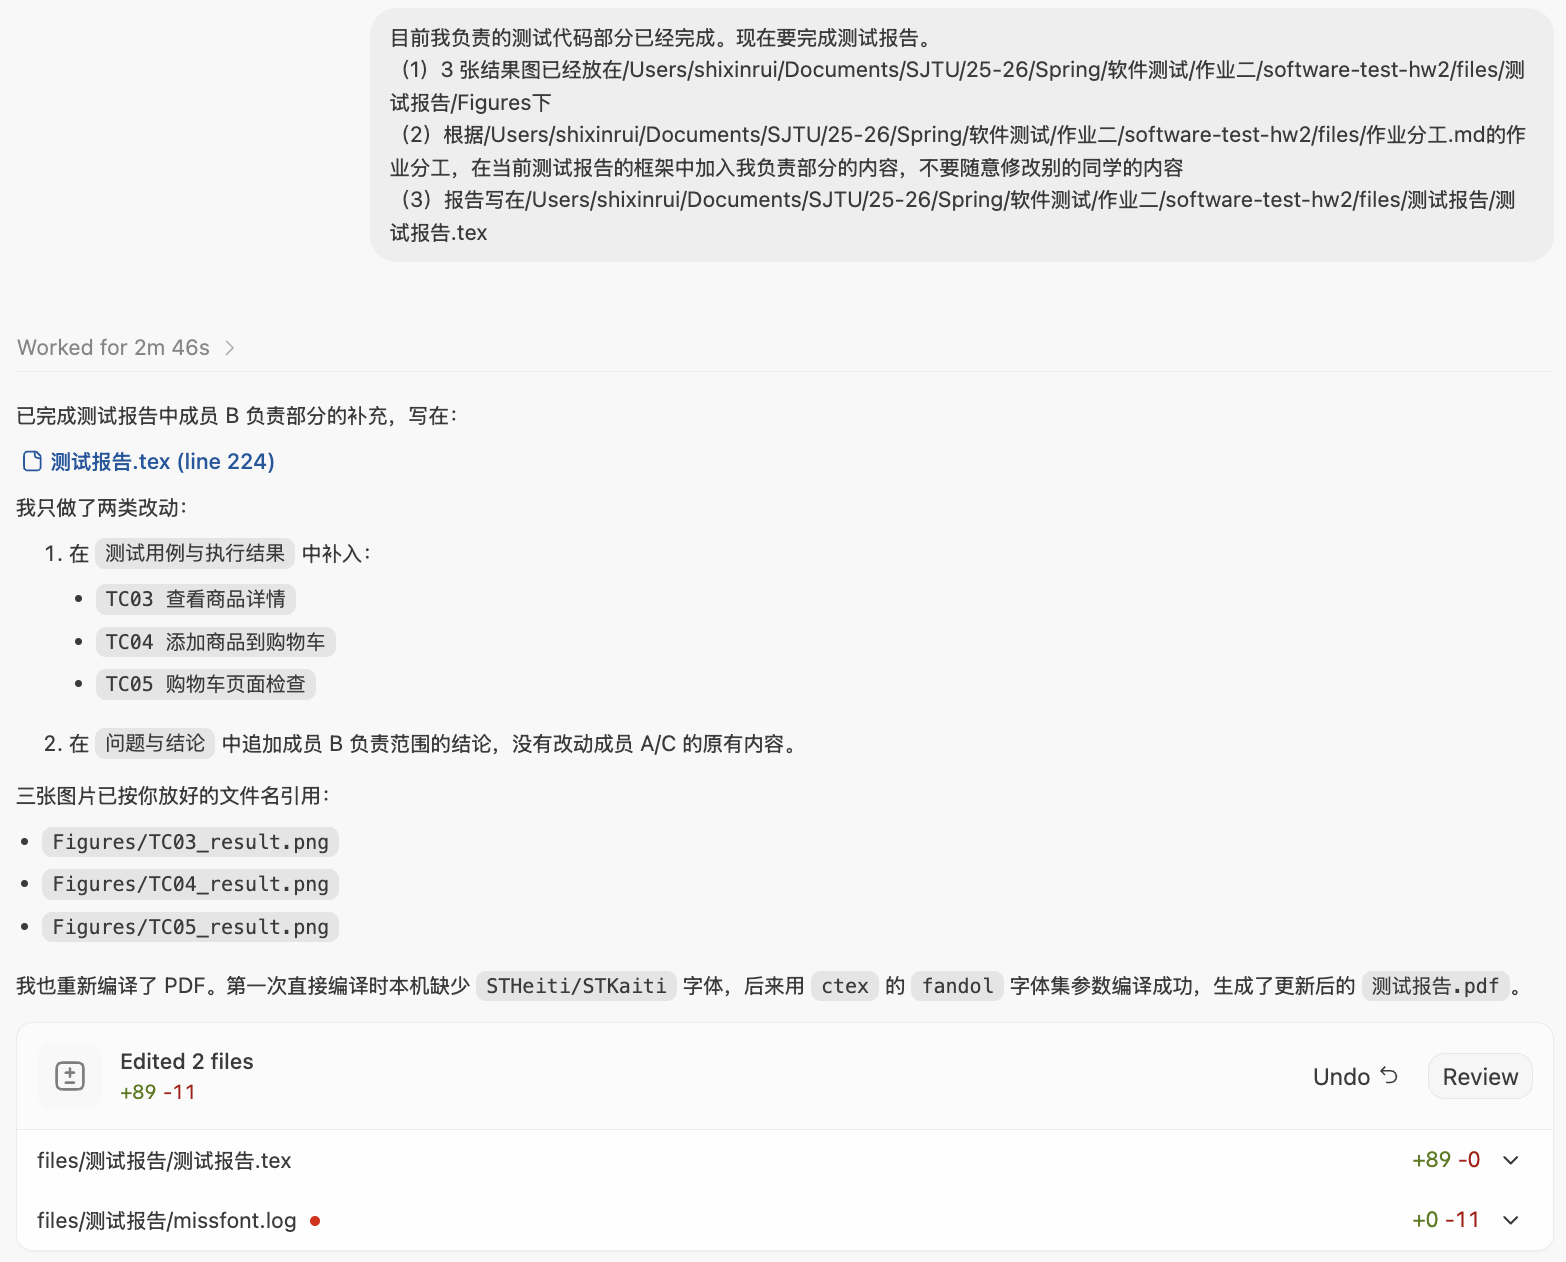
\includegraphics[width=0.92\textwidth]{member_b/测试报告生成.png}
\caption{要求大模型根据分工、测试代码和结果截图，在测试报告中补充成员 B 负责的测试用例与执行结果。}
\end{figure}

\begin{figure}[H]
\centering

\includegraphics[width=0.92\textwidth]{member_b/测试报告修改.png}
\caption{针对测试报告中 TC04 进入商品详情页方式和 TC05 数量表述进行修改，使成员 B 相关内容更清晰。}
\end{figure}

\section{成员C使用记录}

\subsection{Web 端测试代码生成与执行}

\begin{figure}[H]
\centering
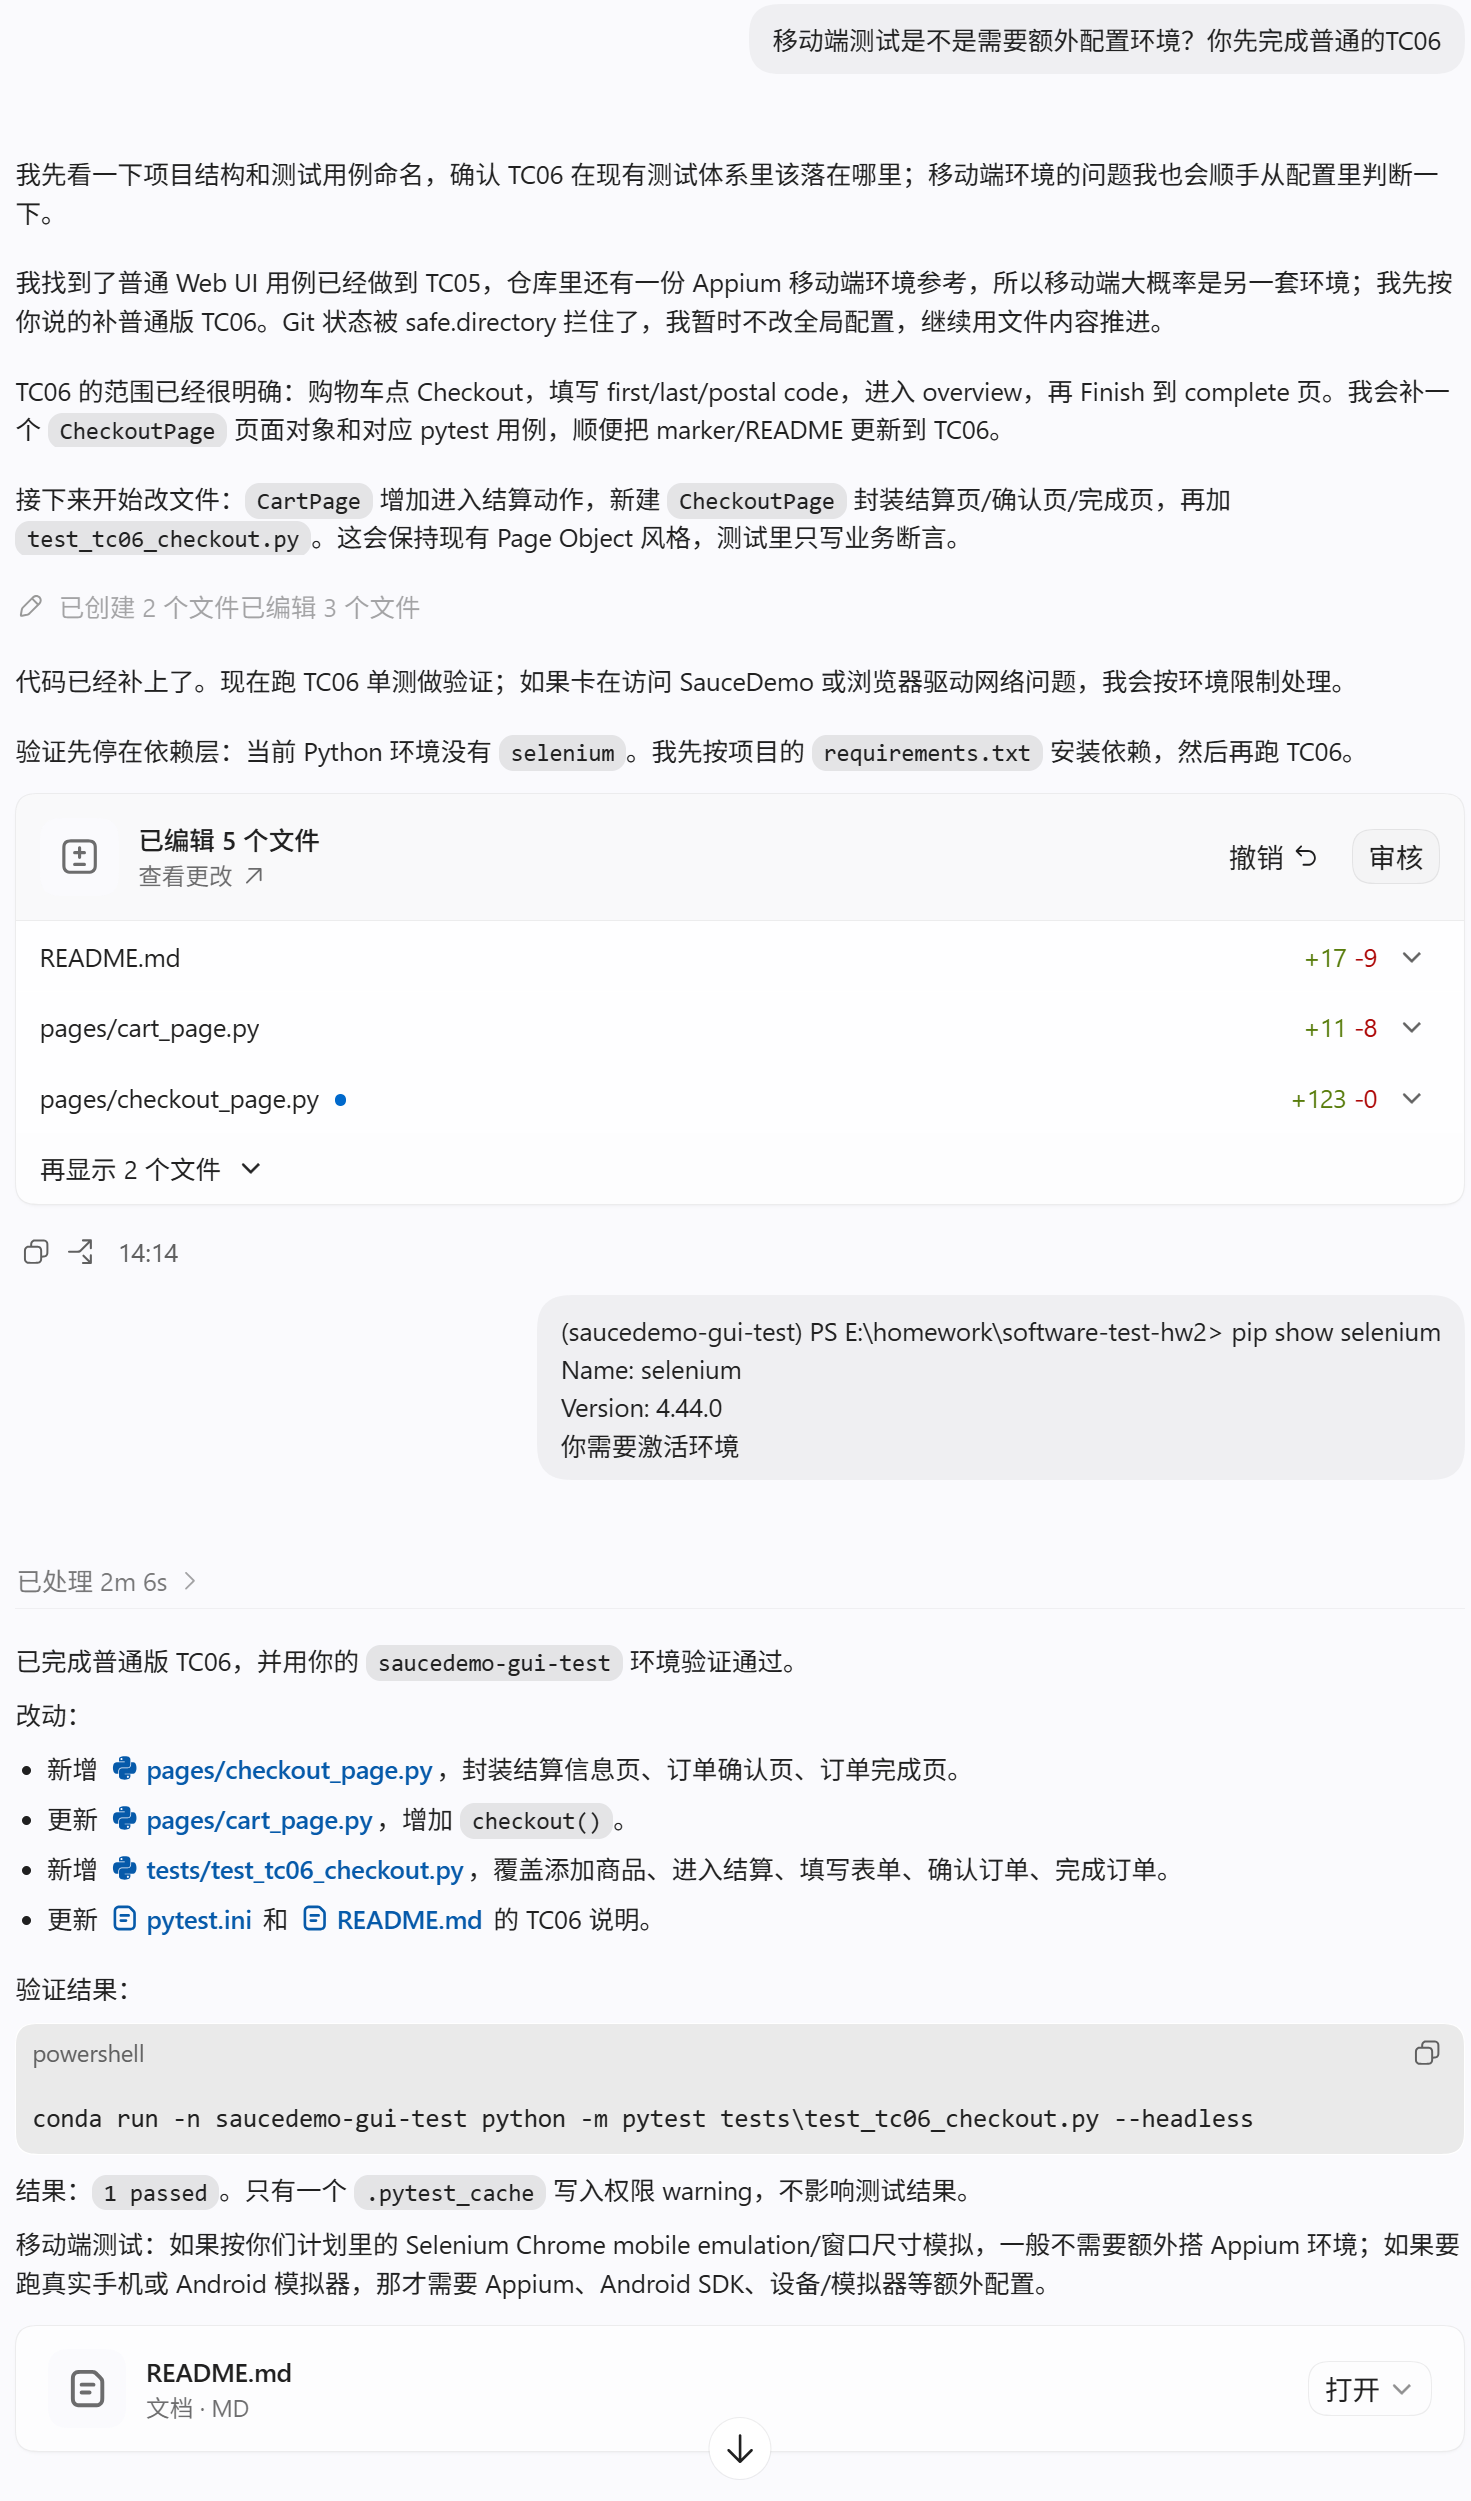
\includegraphics[width=0.92\textwidth,height=0.68\textheight,keepaspectratio]{member_c/web端测试代码生成.png}
\caption{向大模型说明先完成普通 Web 端 TC06 的需求，生成结算与订单完成相关的测试代码和页面对象。}
\end{figure}

\begin{figure}[H]
\centering
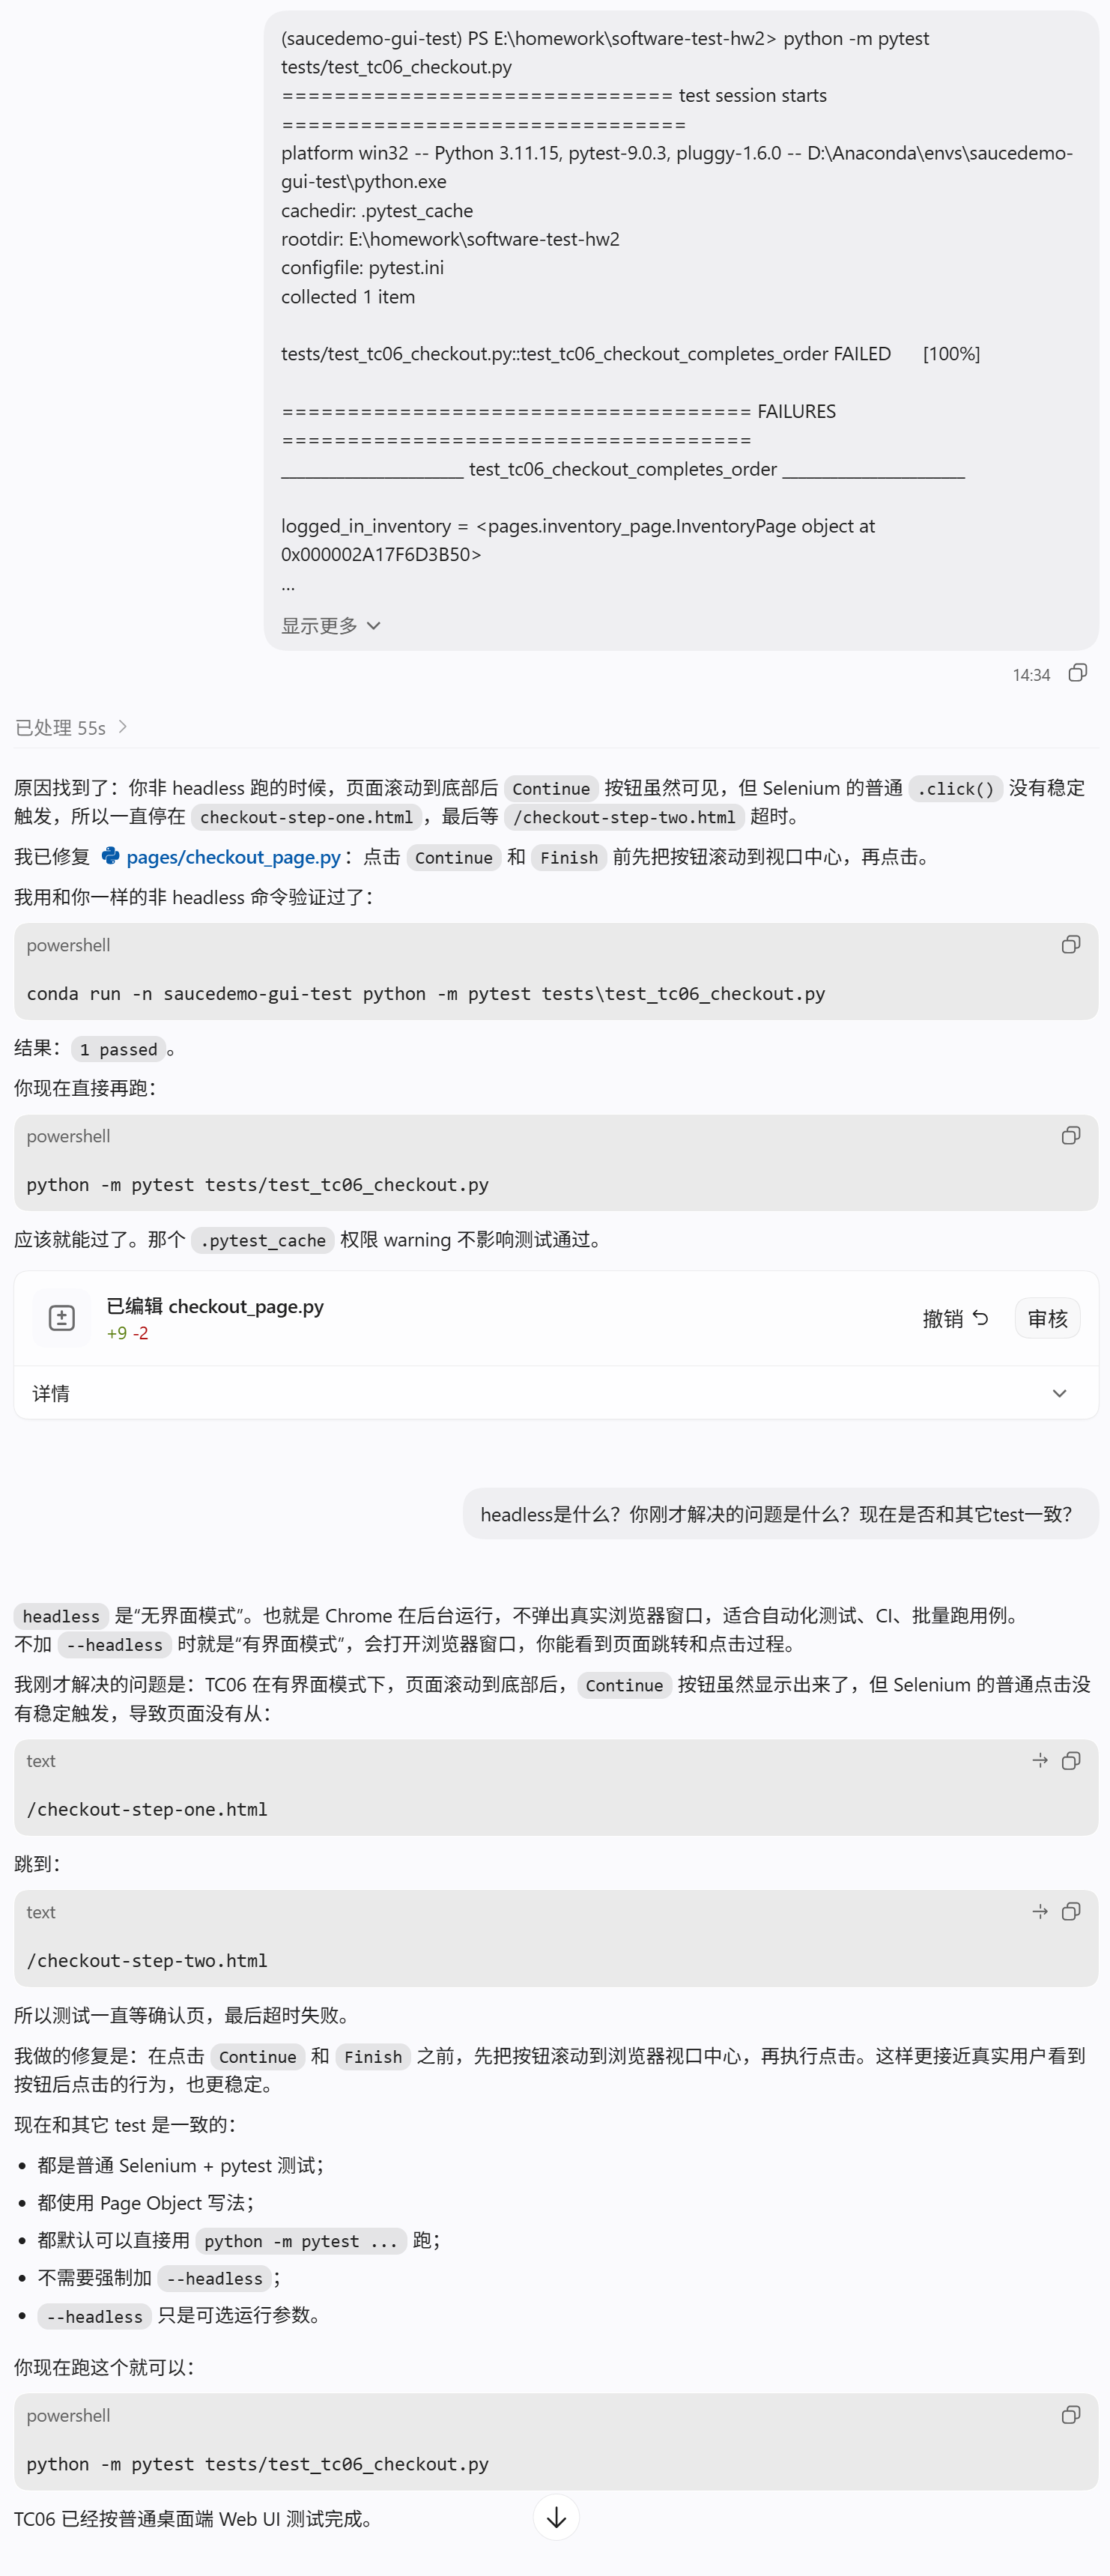
\includegraphics[width=0.92\textwidth,height=0.68\textheight,keepaspectratio]{member_c/web端测试代码修复及运行.png}
\caption{根据本地运行结果，与大模型一起定位 TC06 在非 headless 模式下点击 Continue 不稳定的问题，并通过滚动到按钮后点击的方式修复，最终运行通过。}
\end{figure}

\subsection{移动端测试计划与环境确认}

\begin{figure}[H]
\centering
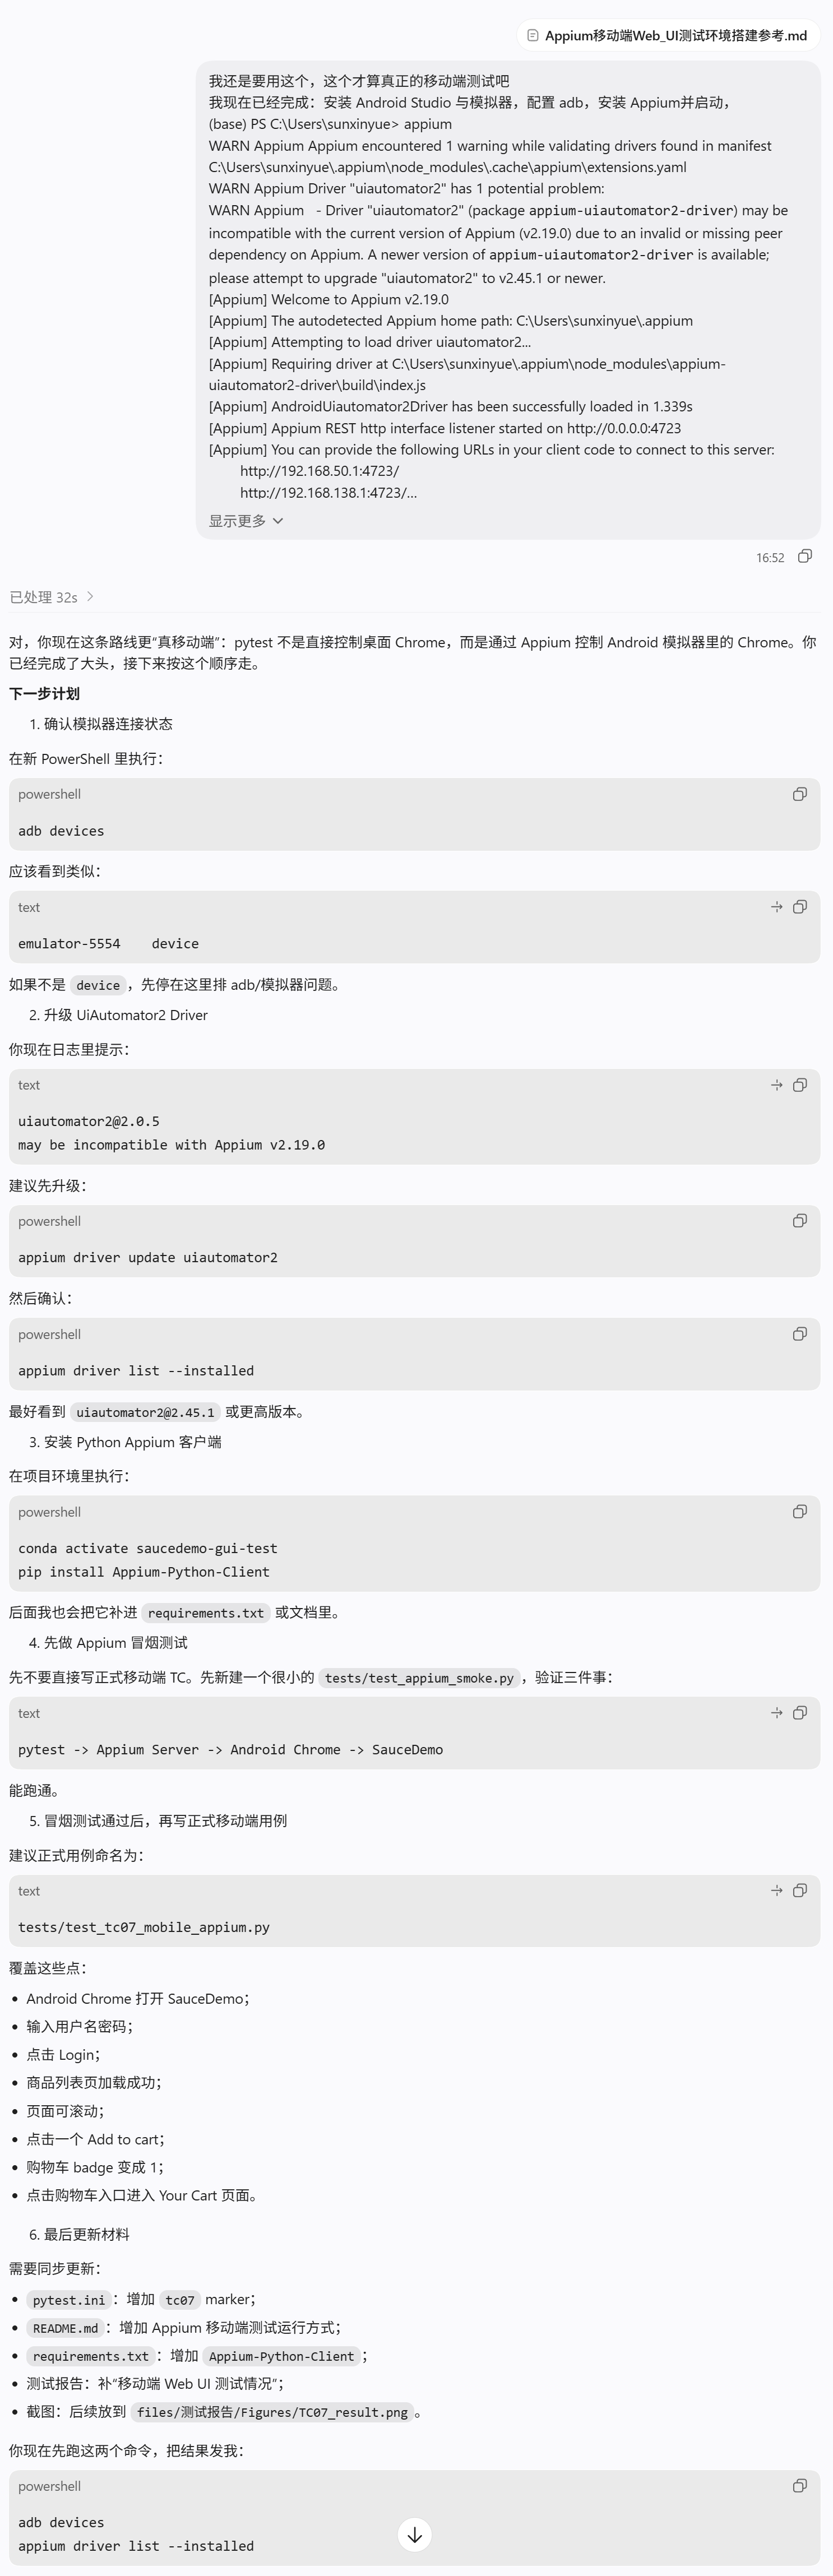
\includegraphics[width=0.92\textwidth,height=0.68\textheight,keepaspectratio]{member_c/移动端测试计划生成.png}
\caption{讨论移动端测试是否需要额外环境，并确定采用 Appium、Android 模拟器和 Android Chrome 进行真实移动端 Web UI 测试。}
\end{figure}

\begin{figure}[H]
\centering
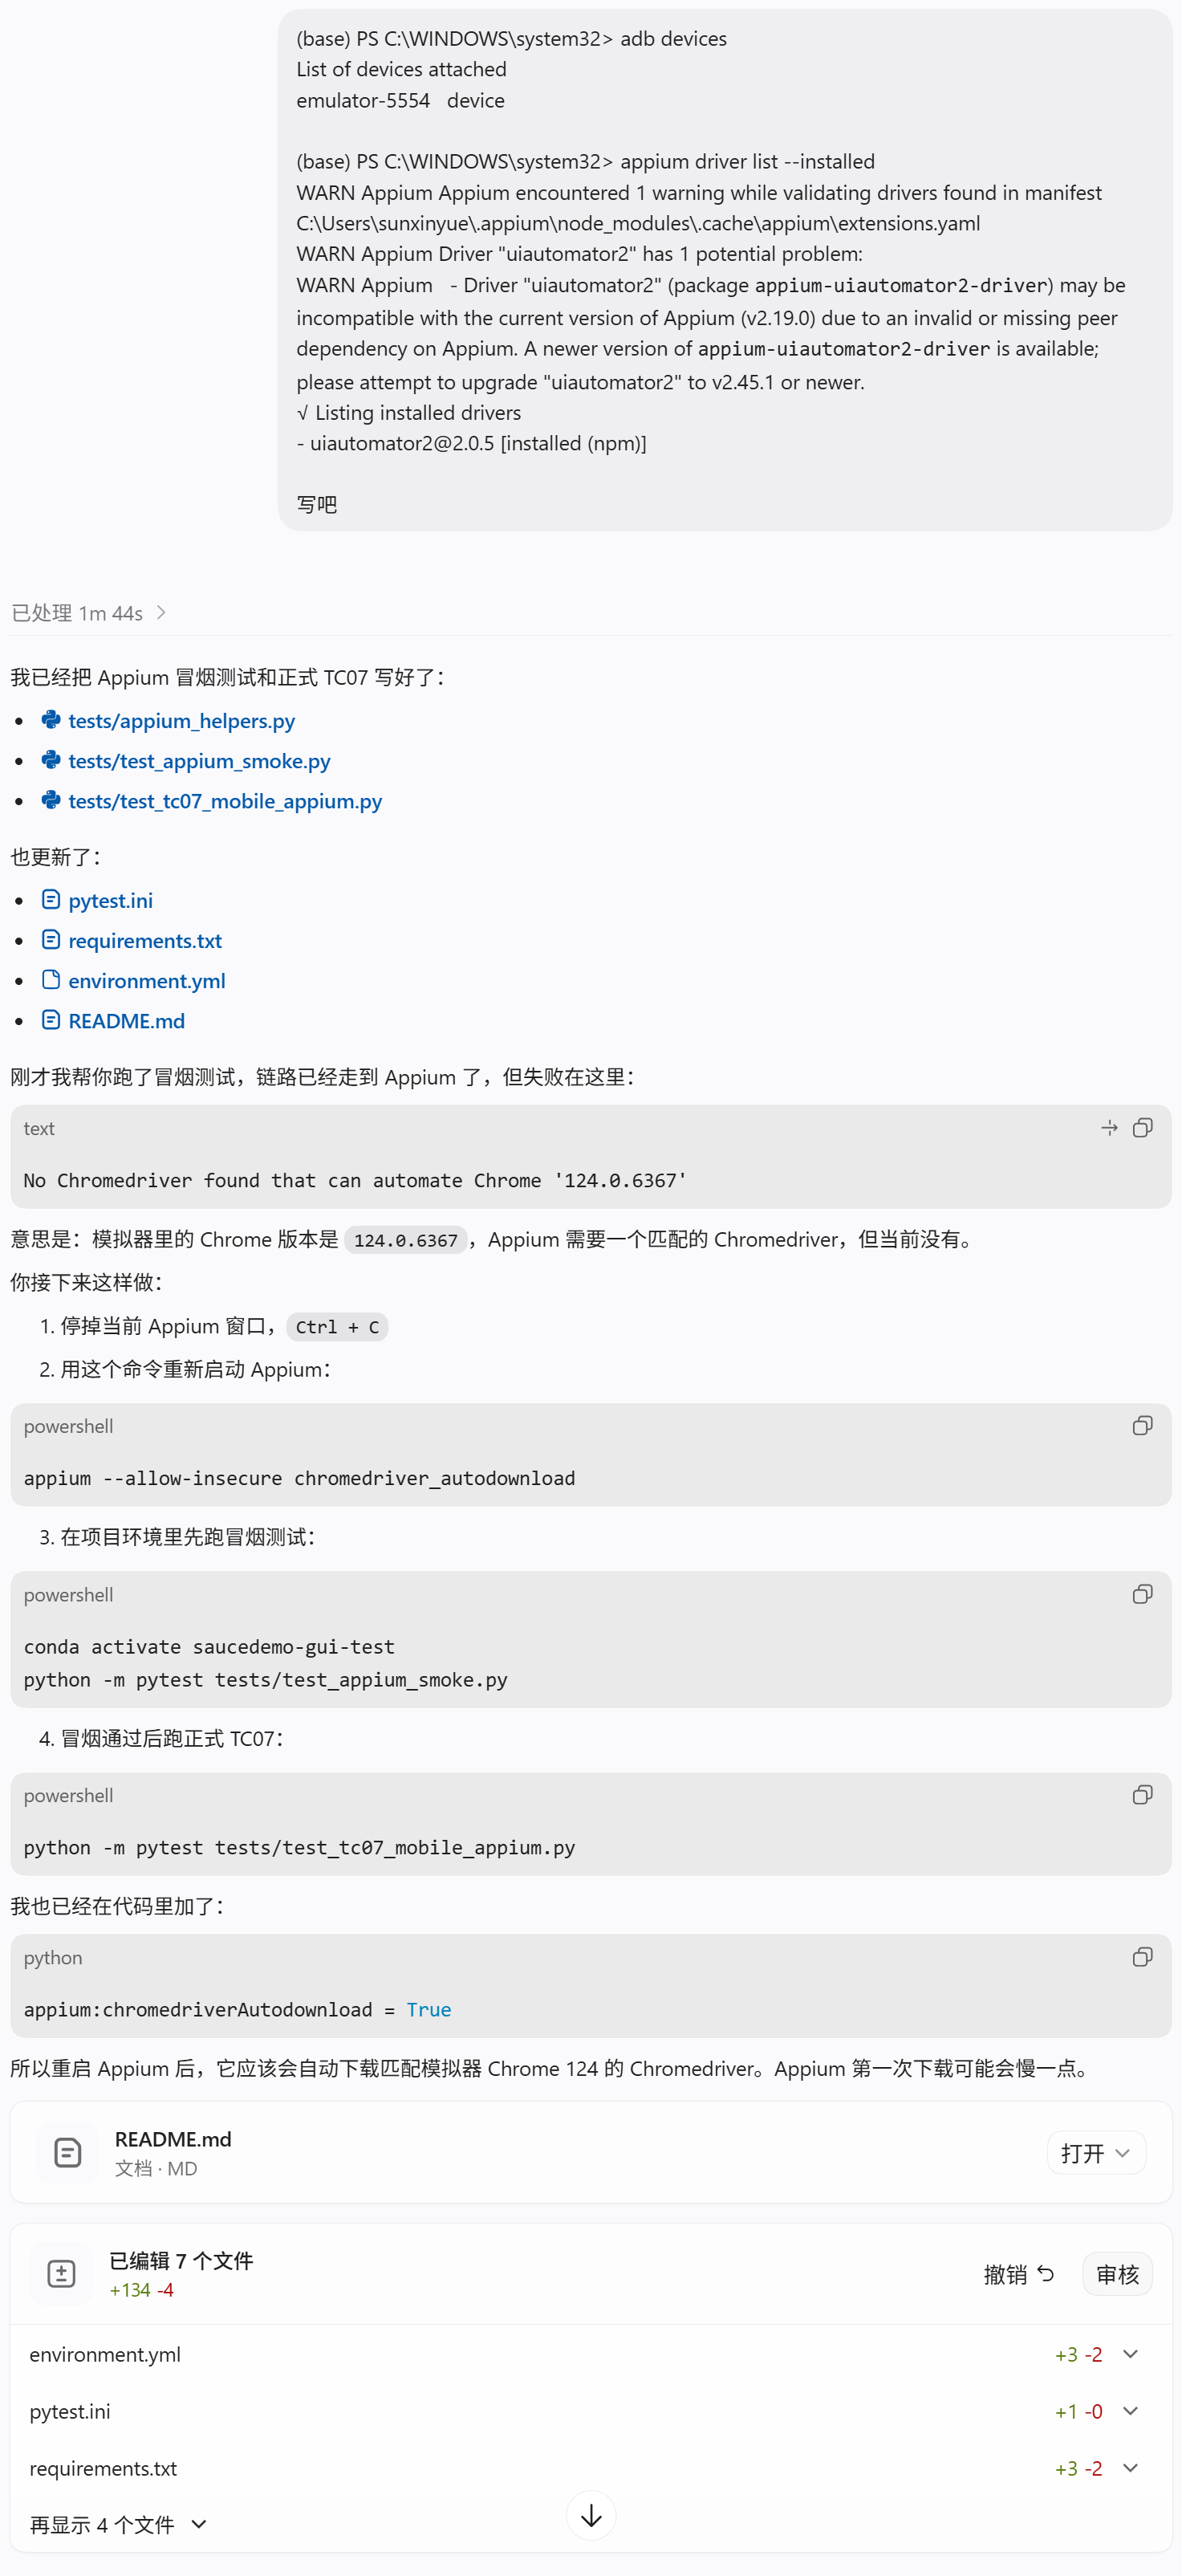
\includegraphics[width=0.92\textwidth,height=0.68\textheight,keepaspectratio]{member_c/移动端测试环境确认及测试代码生成.png}
\caption{在已安装 Android Studio、模拟器、adb 和 Appium 的基础上，向大模型确认后续步骤，并生成 Appium 冒烟测试和移动端测试代码。}
\end{figure}

\subsection{移动端测试错误定位与修复}

\begin{figure}[H]
\centering
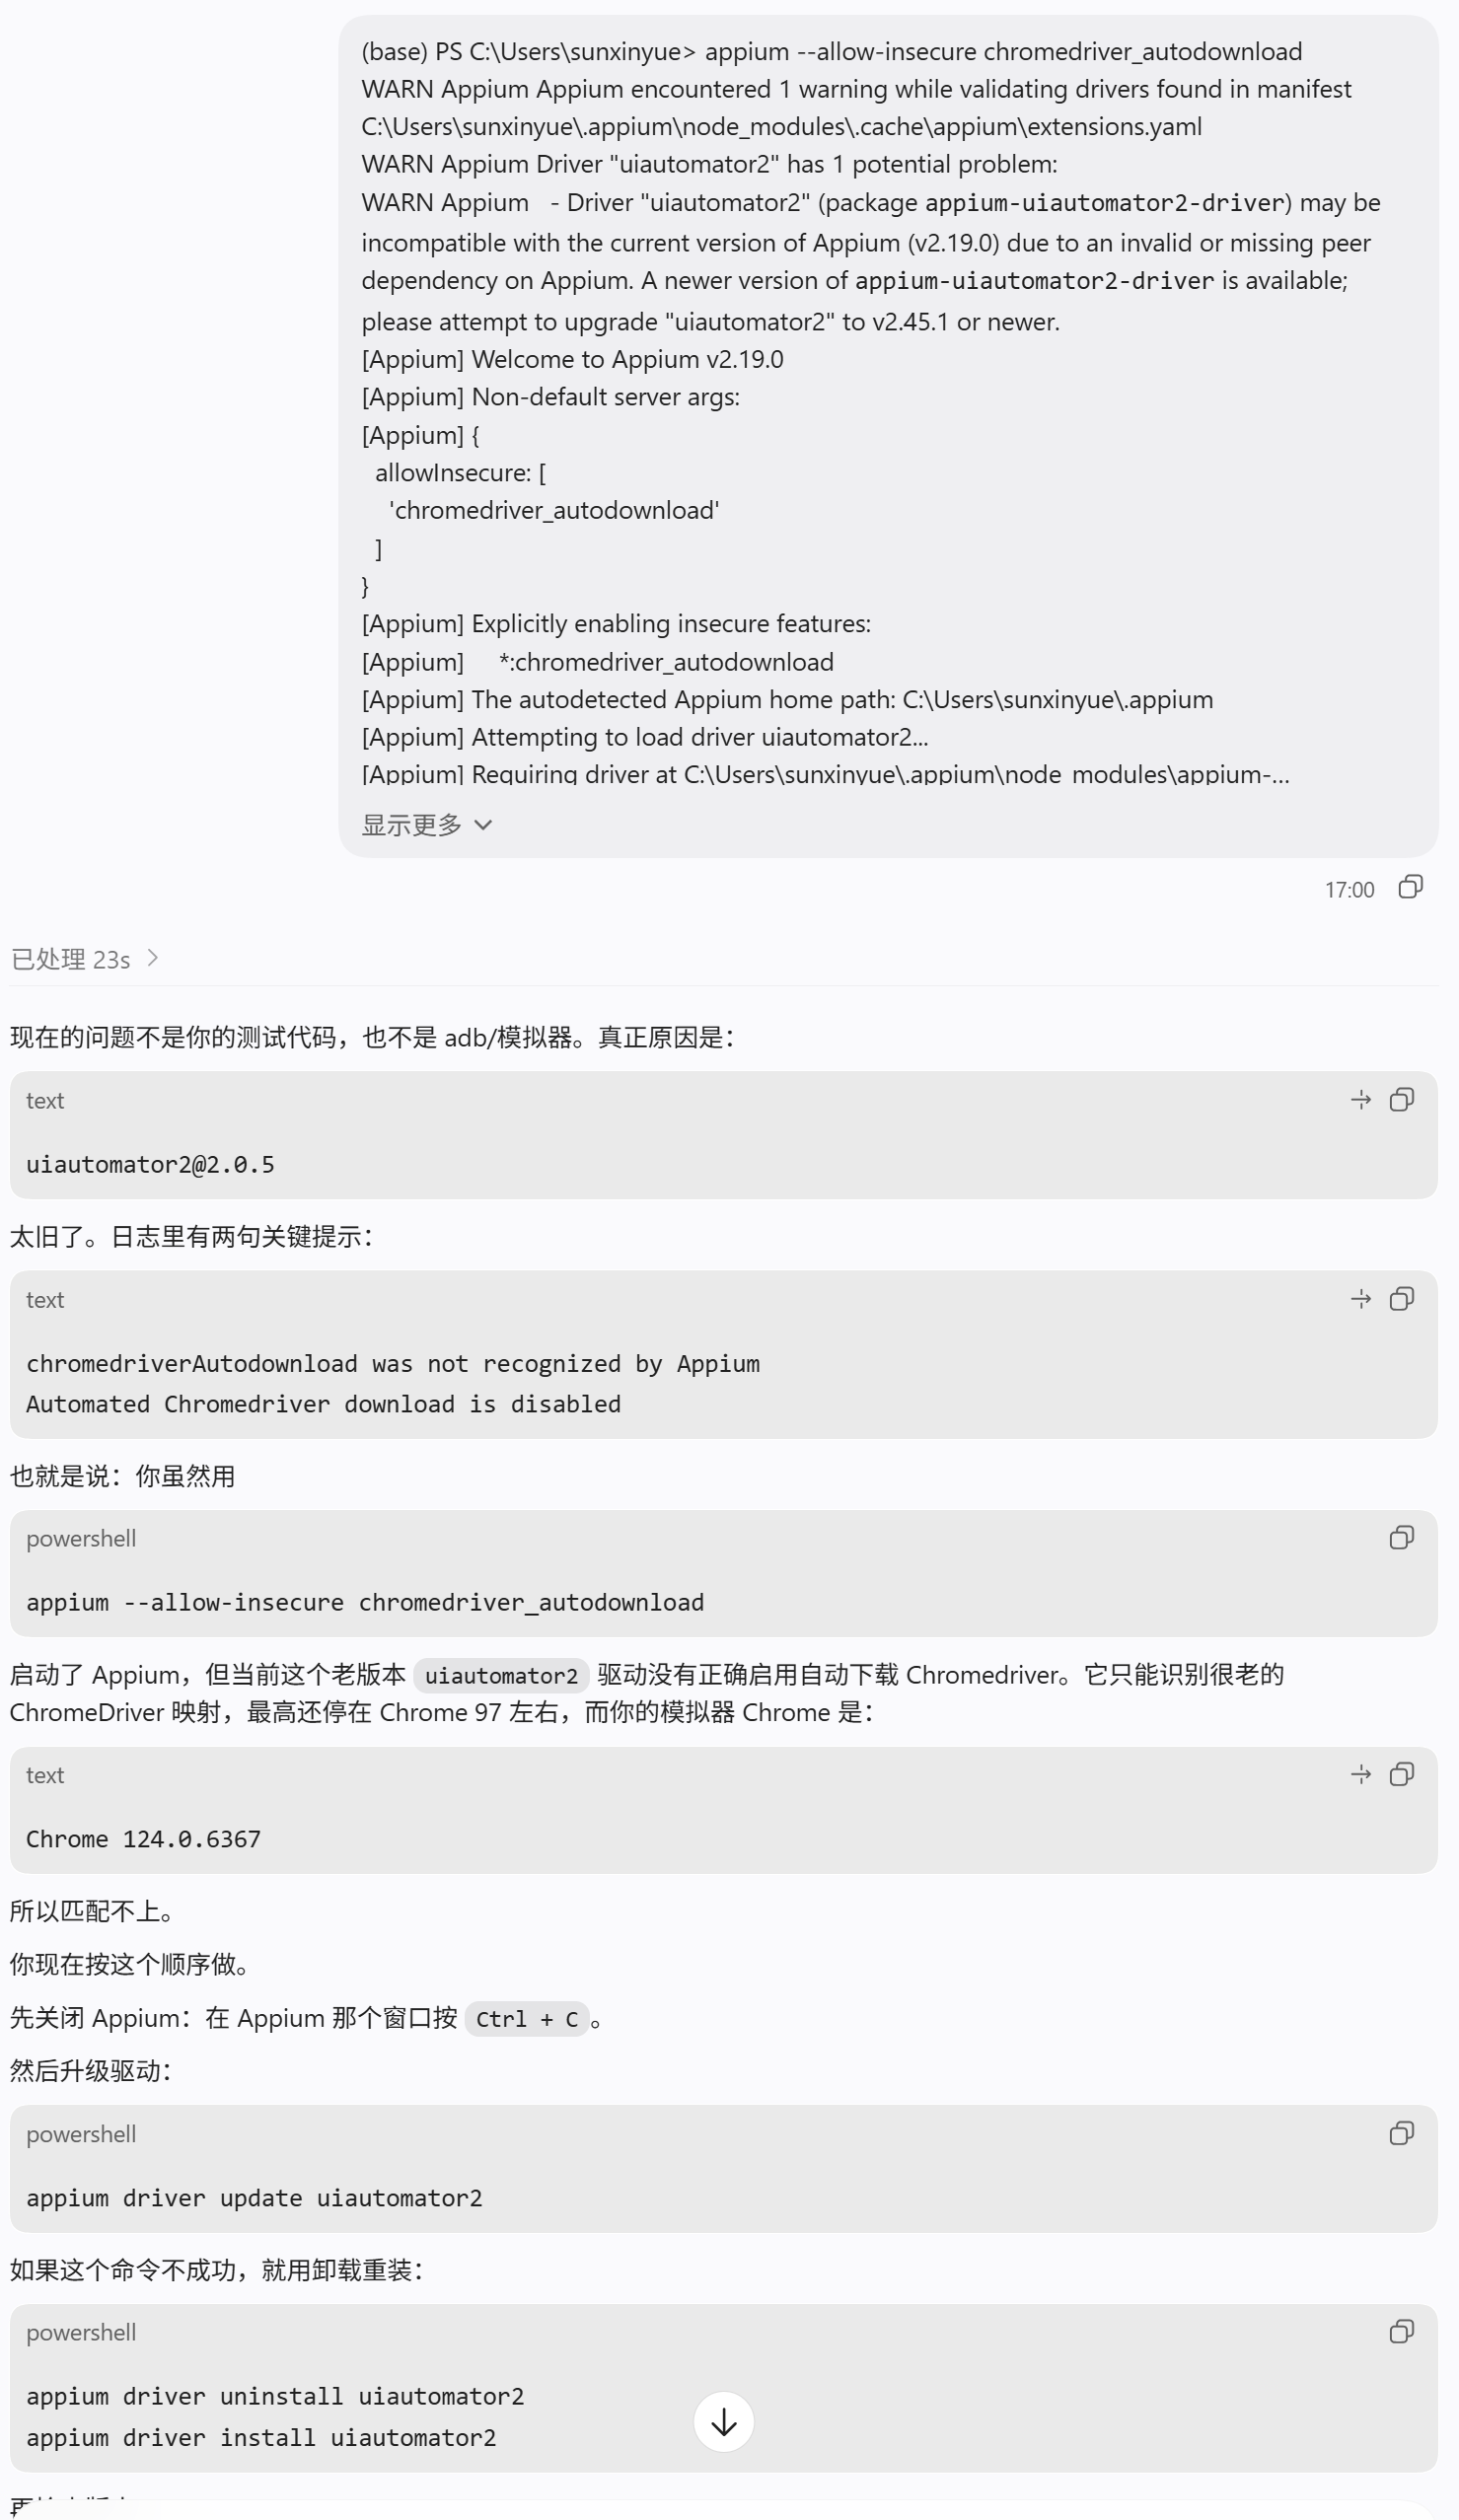
\includegraphics[width=0.92\textwidth,height=0.68\textheight,keepaspectratio]{member_c/移动端测试错误修复1.png}
\caption{运行 Appium 冒烟测试时遇到 Chromedriver 与 Android Chrome 版本不匹配问题，和大模型一起分析原因并调整 Appium 启动方式。}
\end{figure}

\begin{figure}[H]
\centering
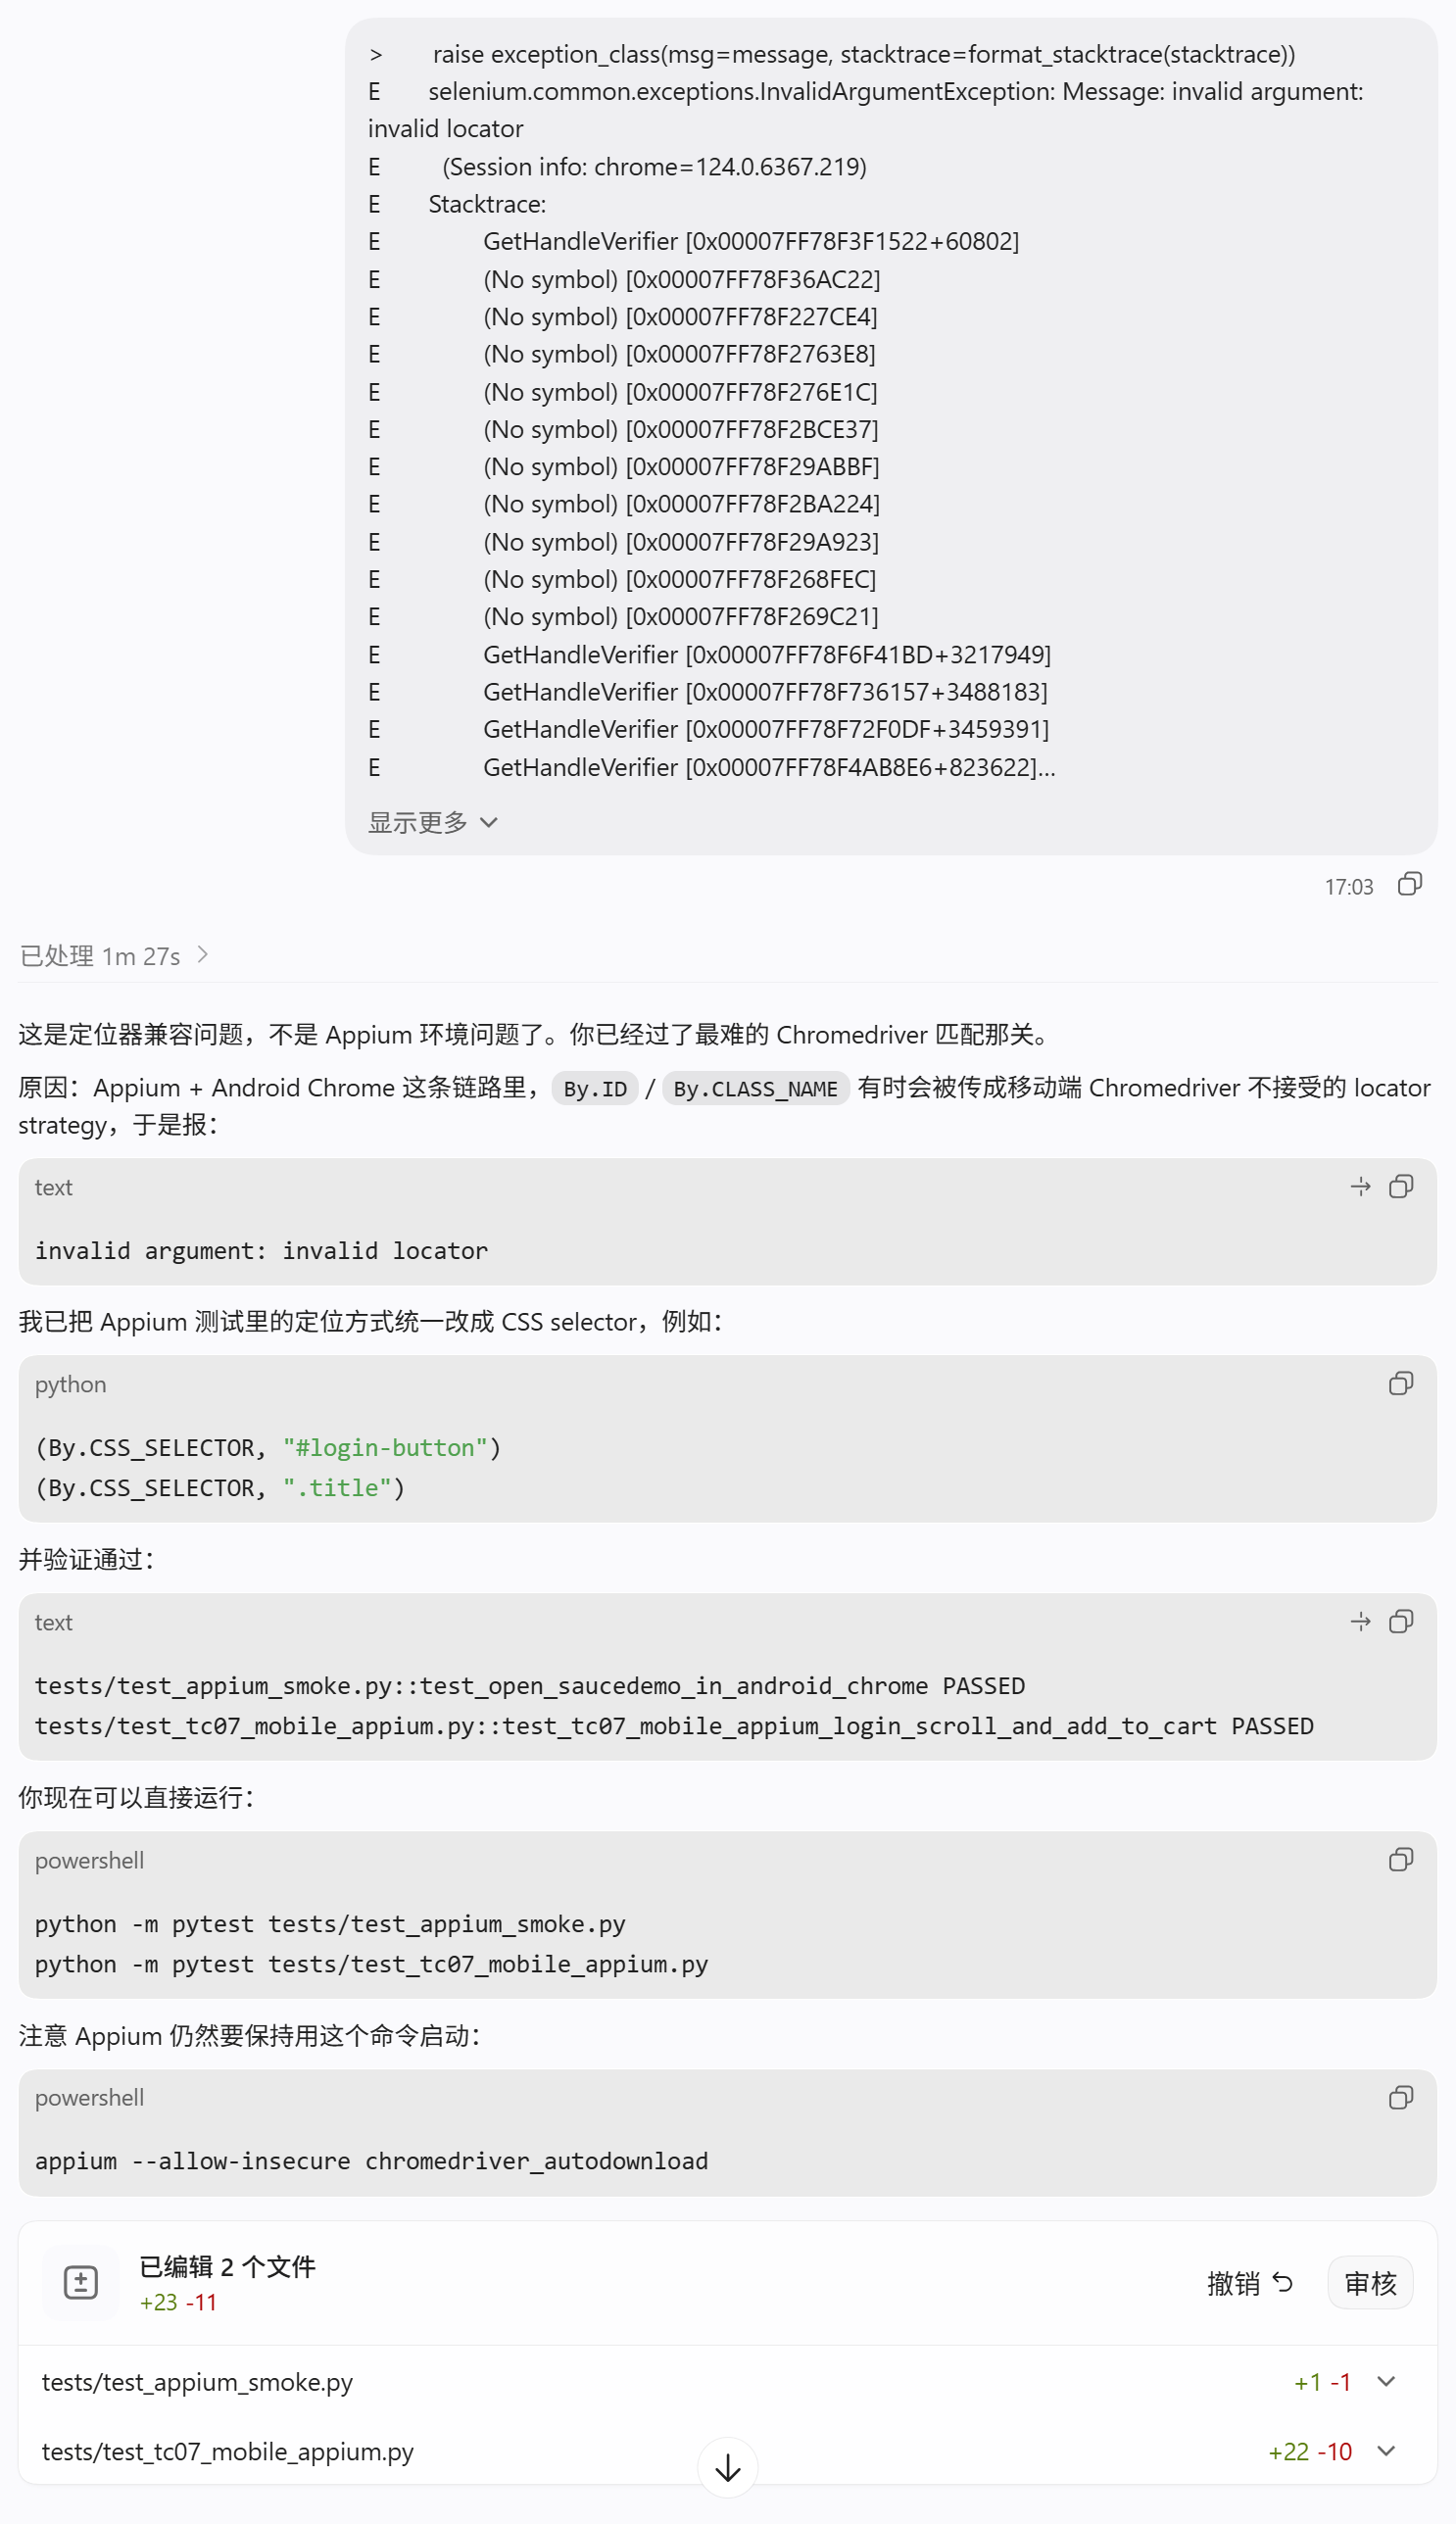
\includegraphics[width=0.92\textwidth,height=0.68\textheight,keepaspectratio]{member_c/移动端测试错误修复2.png}
\caption{继续处理移动端测试中的 locator 兼容问题和点击稳定性问题，将定位方式调整为 CSS selector，并优化移动端页面点击逻辑。}
\end{figure}

\begin{figure}[H]
\centering
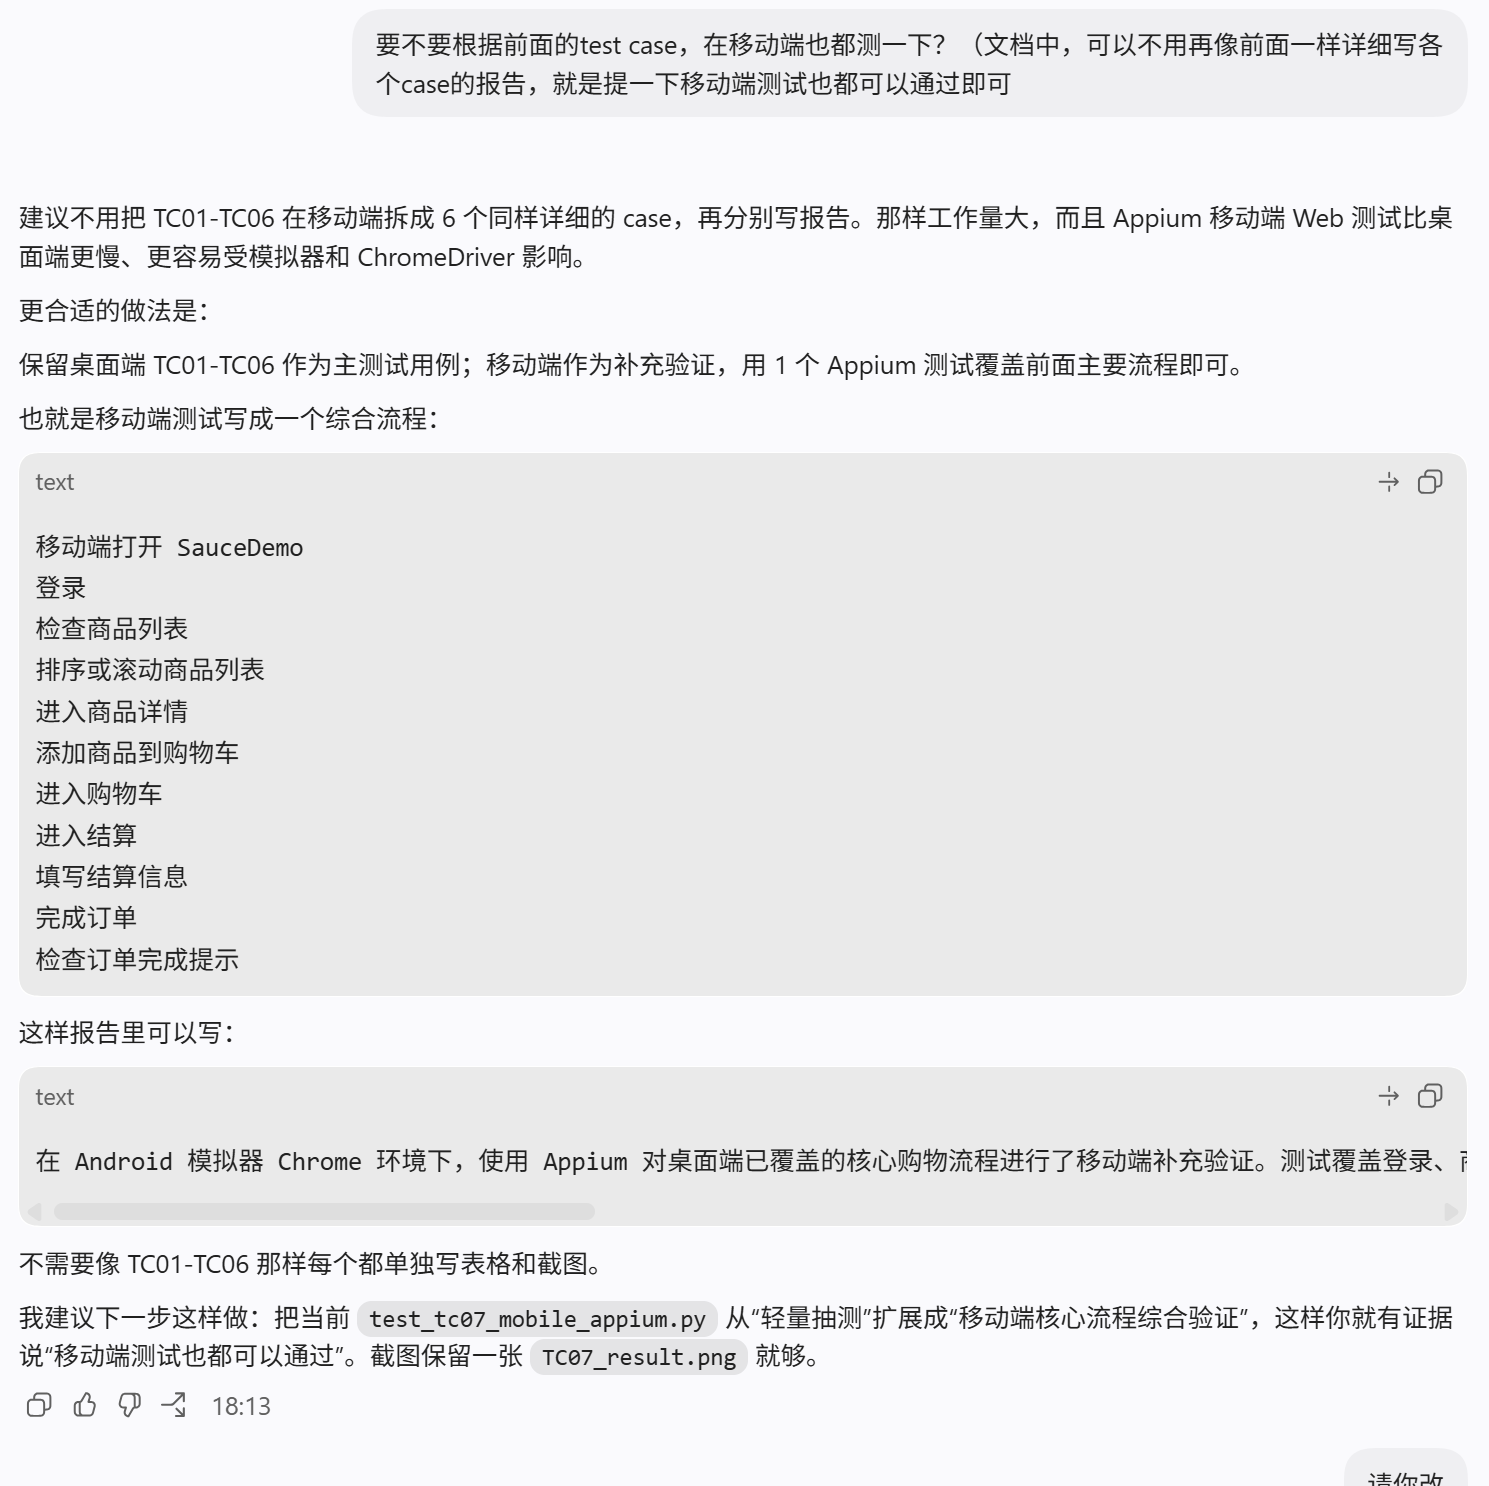
\includegraphics[width=0.92\textwidth,height=0.68\textheight,keepaspectratio]{member_c/商量并调整移动端测试内容.png}
\caption{根据测试计划编号重新梳理 TC07 与移动端测试的关系，将侧边栏导航菜单保留为 TC07，并将 Appium 移动端综合测试调整为 TC08。}
\end{figure}

\subsection{测试报告编写与修改}

\begin{figure}[H]
\centering

\includegraphics[width=0.92\textwidth,height=0.68\textheight,keepaspectratio]{member_c/测试报告生成.png}
\caption{要求大模型根据成员 C 负责的 TC06、TC07 和 TC08 测试内容，在测试报告中补充对应测试步骤、检查点、执行结果和截图引用。}
\end{figure}

\begin{figure}[H]
\centering
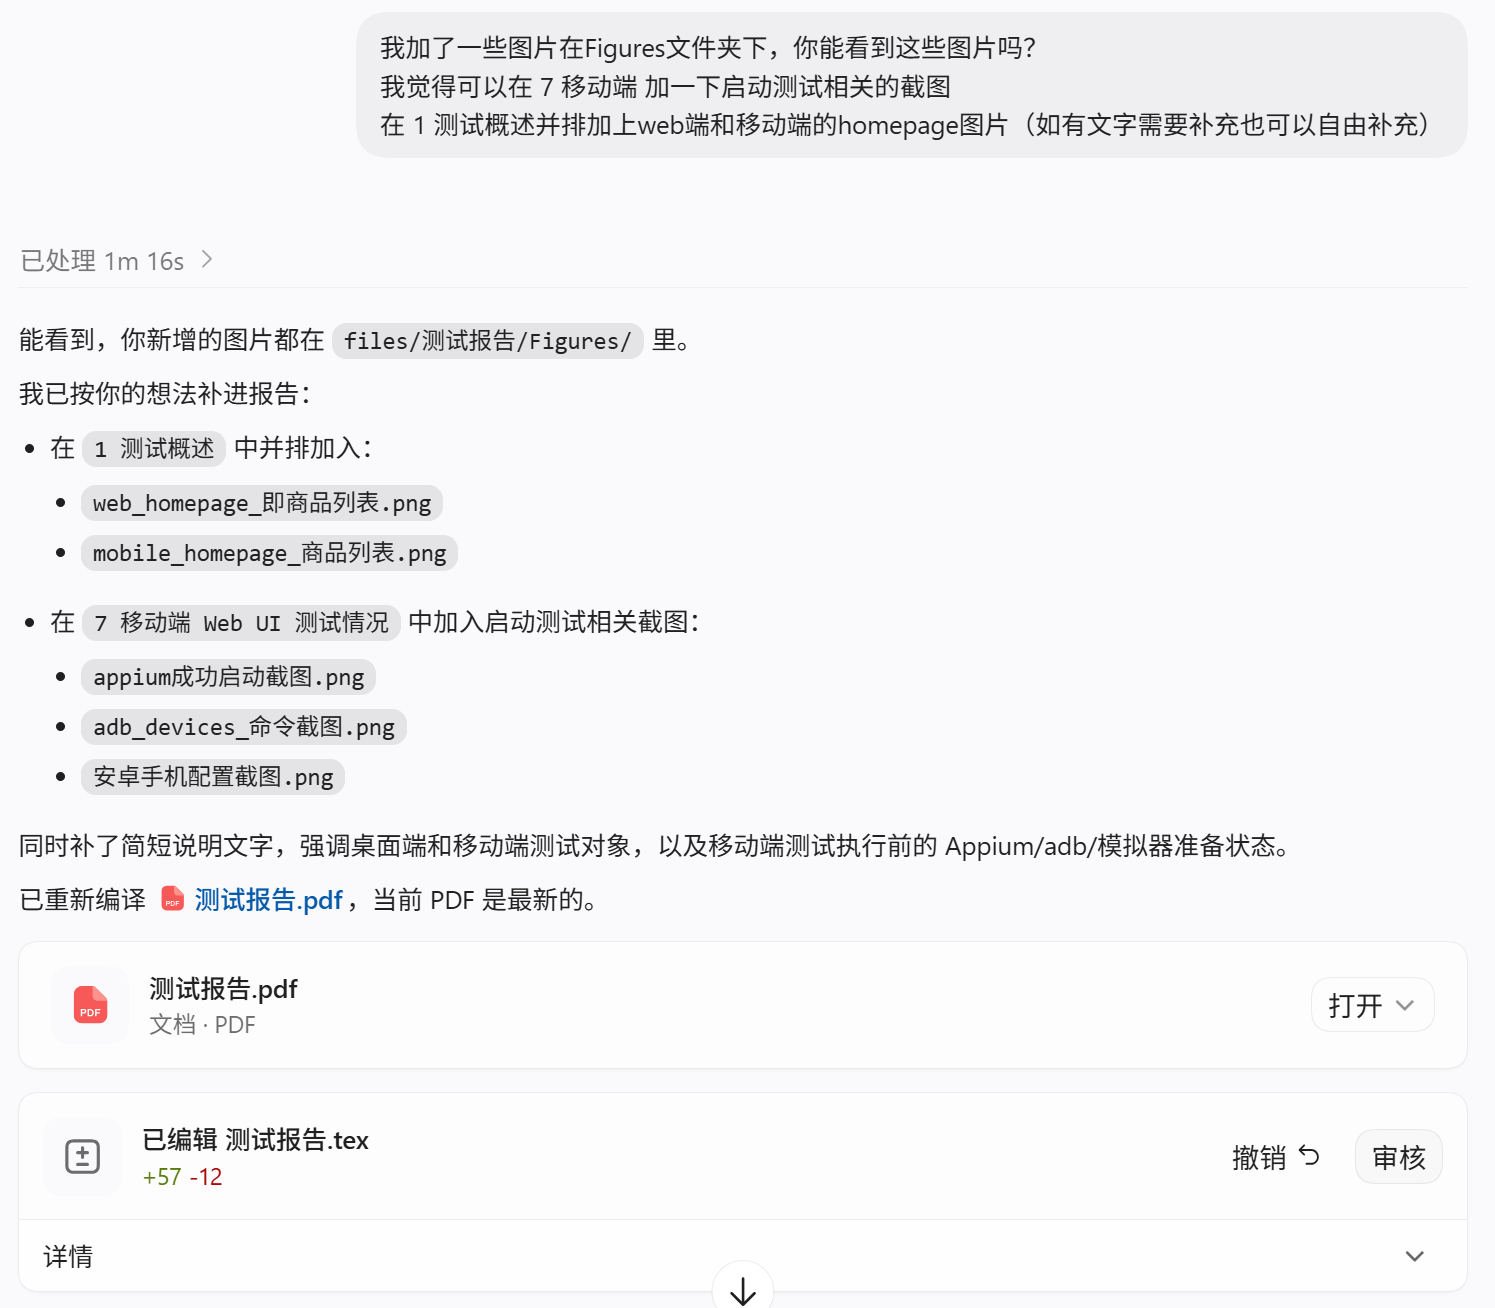
\includegraphics[width=0.92\textwidth,height=0.68\textheight,keepaspectratio]{member_c/测试报告调整.png}
\caption{继续与大模型讨论测试报告结构和表述方式，对桌面端与移动端测试环境、问题与结论、UI 截图展示等内容进行调整。}
\end{figure}

\end{document}
